\section{Elementi di teoria dei numeri}

\subsection{Divisibilità e massimo comun divisore}

\begin{definition}[Divisibilità]
    \label{def:divisibilita}
    Si dice che $d$ divide $a$, e $a$ è multiplo di $d$ se,
    $
    \forall d \ne 0 \in \mathbb{Z}
    ,
    a \in \mathbb{Z}
    $
    \begin{equation*}
        d | a 
        \quad
        \text{se}
        \quad
        \exists k \in \mathbb{Z} : a = kd
    \end{equation*}
\end{definition}
\begin{definition}[Divisore]
    \label{def:divisore}
    Se $d$ divide $a$ e $d>0$ si dice che è divisore di $a$.
    Per esempio $-2$ divide $8$, mentre $2$ è divisore di $8$.
\end{definition}
Valgono le seguenti proposizioni riguardo alla divisibilità:
\begin{proposizione}
    $\forall d \in \mathbb{Z} - \left\{ 0 \right\}
    \Rightarrow
    d | 0$
\end{proposizione}
\begin{proposizione}
    $
    \left( d | a \right)
    \wedge
    \left( a \ne 0 \right)
    \Rightarrow
    |d| \leq |a|
    $
\end{proposizione}
\begin{corollario}
    \label{cor:divisore_limite}
    $
    \left( d | a \right)
    \wedge
    \left( a,d > 0 \right)
    \Rightarrow
    d \leq a
    $
\end{corollario}
\begin{proposizione}
    $
    \left( b | a \right)
    \wedge
    \left( a | b \right)
    \Rightarrow
    a = \pm b
    $ ovvero $
    |a| = |b|
    $
\end{proposizione}
\begin{definition}[Numero primo]
    \label{def:numeroprimo}
    $p > 1$ è primo se ha come divisori solo $1$ e $p$. Il numero $1$ non è considerato primo.
\end{definition}
\begin{theorem}[Divisione]
    \label{teo:divisione}
    Il teorema di divisione garantisce l'esistenza e l'unicità di quoziente e resto.
    \begin{equation*}
        \forall a \in \mathbb{Z}, \forall n \in \mathbb{Z}^+
        \quad
        \exists !
        \;
        q, r :
        a = qn + r
    \end{equation*}
    Dove $q$ è detto il quoziente della divisione intera
    \begin{equation*}
        q \in \mathbb{Z}
        \quad
        q = \left\lfloor 
            \frac{a}{n}
        \right\rfloor
        = a \divv n
    \end{equation*}
    E $r$ è detto resto della divisione intera
    \begin{equation*}
        r \in \mathbb{N}, 0 \leq r < n
        \quad
        r = a \bmod n
    \end{equation*}
\end{theorem}
\begin{corollario}
    Il teorema di divisione prova formalmente quello che si è già visto molto spesso per cui 
    \begin{equation*}
        -1 \bmod n = n-1
        \quad
        -1 = \left( -1 \right) n + \left( n-1 \right)
    \end{equation*}
\end{corollario}
\begin{definition} [Divisori comuni]
    \label{def:divisoricomuni}
    Dati $d > 0, a, b \in \mathbb{Z}$; $d$ è divisore comune di $a$ e $b$ se 
    $d|a$
    e
    $d|b$.
\end{definition}
\begin{proposizione}
    \label{prop:divisore_cli}
    Se $d$ è divisore comune di $a$ e $b$, è anche divisore di ogni loro combinazione lineare intera:
    \begin{equation*}
        \left( 
            d|a
        \right)
        \wedge
        \left( 
            d|b
        \right)
        \Rightarrow
        \forall x, y \in \mathbb{Z} :
        d | ax + by
    \end{equation*}
    \begin{proof}
        $d | a \leftrightarrow \exists k_a : a = k_a d$ 
        e
        $d | b \leftrightarrow \exists k_b : b = k_b d$ 
        allora si riscrive 
        $
        ax + by = k_a d x + k_b d y
        =
        \left( k_a x + k_b y \right) d
        $ e posto $
        k_d = 
        \left( k_a x + k_b y \right)
        $ vale $
        ax + by = k_d d
        $.
    \end{proof}
\end{proposizione}
\begin{definition} [Massimo comun divisore]
    \label{def:gcd}
    Siano $a, b \in \mathbb{Z} : |a| + |b| > 0$
    Il massimo comun divisore (\emph{greatest common divisor} o GCD) di $a$ e $b$ è
    \begin{equation*}
        gcd(a, b) = \max \left\{ 
            d > 0 :
            \left( 
                d|a
            \right)
            \wedge
            \left( 
                d|b
            \right)
        \right\}
    \end{equation*}
    L'ipotesi $|a| + |b| > 0$ garantisce che l'insieme sia limitato.
    Si pone per convenzione
    \begin{equation*}
        gcd(0,0) = 0
    \end{equation*}
\end{definition}
Valgono le seguenti proposizioni riguardo al GCD:
\begin{proposizione}
    \label{prop:gcd_bound}
    $ 
    |a| + |b| > 0
    \Rightarrow 
    1 \leq gcd(a,b)
    \leq \min \left\{ |a|, |b| \right\}
    $
\end{proposizione}
\begin{proposizione}
    \label{prop:gcd_zero}
    $ 
    \forall a \in \mathbb{Z}
    \Rightarrow 
    gcd(a,0) = |a|
    $ (anche per $a=0$ è coerente)
\end{proposizione}
\begin{proposizione}[Sign insensitivity]
    Vale
    \begin{equation*}
        gcd(a,b) =
        gcd(-a,b) =
        gcd(a,-b) =
        gcd(-a,-b) =
        gcd(|a|,|b|)
    \end{equation*}
    Questo permette di limitarsi allo studio dei naturali senza perdita di generalità.
\end{proposizione}

\subsection{Teorema di Bézout}

\begin{theorem} [Identità di Bézout]
    \label{teo:bezout}
    Sotto l'ipotesi $|a| + |b| > 0$, il GCD
    di $a$ e $b$
    è la minima combinazione lineare intera positiva 
    di $a$ e $b$.
    \begin{equation*}
        gcd(a,b) =
        \min \left\{ 
            d > 0 :
            \exists x, y \in \mathbb{Z} :
            d = ax + by
        \right\}
    \end{equation*}
    \begin{proof}
        Si mostra l'uguaglianza $
        gcd(a,b) = s
        $ dimostrando la minorazione e maggiorazione.
        \\
        ``$ gcd(a,b) \leq s $'':
        Per definizione di GCD vale $
        \left( 
            gcd(a,b) | a
        \right)
        \wedge
        \left( 
            gcd(a,b) | b
        \right)
        $
        e per la proprietà \ref{prop:divisore_cli} vale $
        gcd(a,b) 
        | ax + by
        ,
        \forall x, y \in \mathbb{Z}
        $.
        Se divide tutte le combinazioni lineari intere, deve dividere anche $s$:
        $
        gcd(a,b) | s
        $.
        Valgono le ipotesi della proposizione \ref{prop:gcd_bound} ($|a| + |b| > 0$), quindi $
        gcd(a,b) > 0
        $.
        Anche $s>0$ perché è il minimo di un insieme di numeri positivi.
        Entrambe le quantità sono positive e la prima divide la seconda, per cui dalla divisibilità discende $
        gcd(a,b) \leq s
        $ (corollario \ref{cor:divisore_limite}).
        \\
        ``$ gcd(a,b) \geq s $'':
        Prima di mostrare la minorazione, occorre dimostrare che
        \begin{equation*}
            \forall x, y \in \mathbb{Z}
            ,
            \;\;
            s | ax + by
        \end{equation*}
        Sia $
        s = a \bar{x} + b \bar{y}
        $ la combinazione minima e $
        c = ax + by
        $ una combinazione generica, si applica il teorema di divisione tra $c$ e $s$:
        \begin{equation*}
            \exists ! q, r :
            c = qs + r
            ,
            \quad
            0 \leq r < s
        \end{equation*}
        va mostrato che deve valere $r=0$, e quindi $s$ divide $c$.
        Si riscrive
        \begin{align*}
            r &= 
            c - qs
            \\
            &= 
            ax + by - q\left( 
                a \bar{x} + b \bar{y}
            \right)
            \\
            &= 
            a \left( 
                x - q \bar{x}
            \right)
            +
            b \left( 
                y - q \bar{y}
            \right)
            \\
            &=
            ax' + by'
        \end{align*}
        E si è mostrato che $r$ è combinazione lineare intera di $a$ e $b$.
        Ma $s$ era il minimo delle combinazioni lineari intere positive, quindi $r$ (che può assumere valori $
            0 \leq r < s
        $) non può essere positivo, perché avrebbe valore inferiore a $s$, e deve essere $r=0$.
        \\
        Avendo mostrato che $s$ divide ogni combinazione lineare intera, se ne possono scegliere due particolari:
        \begin{equation*}
            s | a \cdot 1 + b \cdot 0 = a
            \quad
            \text{e}
            \quad
            s | a \cdot 0 + b \cdot 1 = b
        \end{equation*}
        Ossia $s$ è divisore comune, minore o uguale al \emph{massimo} comun divisore: $
        gcd(a,b) \geq s 
        $.
    \end{proof}
\end{theorem}

\subsection{Teorema di Euclide}

Per il calcolo efficace del GCD si utilizza l'algoritmo di Euclide, considerato il primo esempio di algoritmo efficiente della storia.

\begin{theorem} [Euclide]
    \label{teo:euclide}
    Siano $a,b \geq 0$ (il GCD è invariante per segno, non si perde di generalità), allora
    \begin{align*}
        b=0
        &
        \Rightarrow
        gcd(a,b) =
        gcd(a,0) = a
        \\
        b>0
        &
        \Rightarrow
        gcd(a,b) =
        gcd(b,
            a \bmod b
        )
    \end{align*}
    \begin{proof}
        La prima implicazione è corrispondente alla proposizione \ref{prop:gcd_zero}.
        \\
        La seconda si prova in due parti:
        \\
        ``$ gcd(a,b) \leq gcd(b, a \bmod b) $'':
        Si applica il teorema di divisione ad $a$ e $b$:
        \begin{equation*}
            a = qb + r = qb + a \bmod b
            \quad
            \rightarrow
            \quad
            a \bmod b = a - qb
        \end{equation*}
        E si riscrive quindi
        \begin{align*}
            gcd(b, a \bmod b)
            &= 
            gcd(b, a - qb)
            % \intertext{a cui si applica il teorema di Bézout:
            % $ \exists x', y' \in \mathbb{Z} : $
            % }
            \\
            \text{per Bézout:
            $ \exists x', y' \in \mathbb{Z} : $
            }
            \quad
            &
            =
            b x' + 
            \left( 
                a - qb
            \right) y'
            \\
            &= 
            a y'
            +
            b
            \left( 
                x' - qy'
            \right)
        \end{align*}
        Per cui il $
        gcd(b, a \bmod b)
        $ è combinazione lineare intera positiva di $a$ e $b$ e sempre per Bézout, deve essere maggiore o uguale del $
        gcd(a, b)
        $, che è la minima combinazione lineare intera positiva:
        $ gcd(a,b) \leq gcd(b, a \bmod b) $.
        \\
        ``$ gcd(a,b) \geq gcd(b, a \bmod b) $'':
        Sia $
        d' = gcd(b, a \bmod b)
        $, allora valgono
        \begin{align*}
            d' | b 
            \Rightarrow
            \exists k' 
            &
            : b = k' d'
            \\
            d' | a \bmod b
            \Rightarrow
            \exists k'' 
            &
            : a \bmod b = k'' d'
        \end{align*}
        E si riscrive dal teorema di divisione
        \begin{align*}
            a
            &= 
            qb + a \bmod b
            \\
            &= 
            q k' d' 
            +
            k'' d'
            \\
            &= 
            \left( 
                q k' + k''
            \right) d'
        \end{align*}
        Quindi $
        \left( d' | a \right)
        $ e chiaramente $
        \left( d' | b \right)
        $, per cui $d'$ è divisore comune di $a$ e $b$, e deve essere minore del \emph{massimo} comun divisore.
    \end{proof}
\end{theorem}
Questo teorema mostra una chiara proprietà di sottostruttura, che riscrive la soluzione in funzione di istanze più piccole del problema.
\begin{algorithm}[H]
\caption{Algoritmo di Euclide}\label{alg:euclide}
\begin{algorithmic}[1]
    \Procedure{Euclid}{$a, b$}
        \If{$b = 0$}
            \State return $a$
        \EndIf
        \State return \Call{Euclid}{$b, a \bmod b$}
    \EndProcedure
\end{algorithmic}
\end{algorithm}
Se $a < b$ la prima iterazione scambia i valori ($
    a \bmod b = a
$), e alle successive iterazioni vale $b < a$ e quindi $a \bmod b < b$, essendo un minore stretto l'algortimo termina.
La correttezza dell'algoritmo è assicurata dal teorema precedente.

Per l'analisi della complessità, vanno introdotti i numeri di Fibonacci.
\begin{definition}
    [Numeri di Fibonacci]
    \label{def:numerifibonacci}
    I numeri di Fibonacci sono definiti come
    \begin{align*}
        F_1 &= 1
        \\
        F_2 &= 1
        \\
        F_{k+1}
        &=  
        F_{k} +
        F_{k-1}
        \quad
        \text{per}
        \quad
        k \geq 2
    \end{align*}
    Il cui valore è calcolabile in formula chiusa:
    \begin{align*}
        F_k &= 
        \frac{1}{
            \sqrt{5}
        }
        \left( 
            \frac{1 + 
                \sqrt{5}
            }{2}
        \right)^{k}
        -
        \frac{1}{
            \sqrt{5}
        }
        \left( 
            \frac{1 -
                \sqrt{5}
            }{2}
        \right)^{k}
        \\
        &
        \geq
        \frac{1}{
            2 \sqrt{5}
        }
        \left( 
            \frac{1 + 
                \sqrt{5}
            }{2}
        \right)^{k}
    \end{align*}
    I numeri di Fibonacci crescono come un esponenziale.
\end{definition}
Supponendo di conoscere il numero di chiamate $k$ eseguite dall'algoritmo di Euclide,
si trovano dei limiti inferiori per la grandezza dei parametri iniziali, dimostrando la velocità di convergenza dell'algoritmo.
% allora si dimostra che i parametri iniziali erano grandi rispetto al numero di chiamate.
\begin{lemma}
    \label{lem:euclide_iterazioni}
    Sia $k$ il numero di chiamate eseguite dall'algoritmo di Euclide, e siano $
    a > b > 0
    $, allora $
    a \geq F_{k+2}
    $ e $
    b \geq F_{k+1}
    $
    \begin{proof}
        La restrizione sugli input non è restrittiva:
        \begin{itemize}[noitemsep,parsep=0pt,partopsep=0pt,topsep=0pt]
            \item nel caso $a<b$ i valori vengono scambiati alla prima iterazione
            \item nel caso $a=b$ l'algortimo termina in due chiamate
            \item nel caso $b=0$ l'algortimo termina in una chiamata
        \end{itemize}
        I limiti si provano per induzione su $k$:
        \\
        Per $k=1$, vale 
        \begin{align*}
            a > b > 0
            \quad
            &
            \rightarrow
            b \geq 1 = F_2
            \\
            &
            \rightarrow
            a \geq 2 = F_3
        \end{align*}
        \\
        Sia vera l'ipotesi induttiva per $k-1$.
        \\
        Si analizza $\text{\textsc{Euclid}}(a,b)$ per $k>1$.
        $\text{\textsc{Euclid}}(b, a \bmod b)$ farà allora $k-1$ chiamate, e vale l'ipotesi induttiva:
        \begin{equation*}
            b \geq F_{(k-1)+2} = F_{k+1}
            \quad
            \text{e}
            \quad
            a \bmod b \geq F_{(k-1)+1} = F_{k}
        \end{equation*}
        Vale $a>b$ quindi per il teorema di divisione
        \begin{align*}
            a &= qb + a \bmod b
            \\
            \left( 
                q = \left\lfloor 
                    \frac{a}{b}
                \right\rfloor \geq 1
            \right)
            \quad 
            \quad 
            \quad 
            &
            \geq
            b + a \bmod b
            \\
            &
            \geq
            F_{k+1}
            +
            F_{k}
            \\
            &= 
            F_{k+2}
        \end{align*}
    \end{proof}
\end{lemma}
Avendo provato questo lemma, sia $
\bar{k}
$ il primo valore (minimo) per cui $
b < F_{
    \bar{k} + 1
}
$, allora $
b \geq F_{
    \bar{k}
}
$ e l'algoritmo non può fare più di $
\bar{k}
$ chiamate.
\begin{align*}
    b
    &
    \geq F_{
        \bar{k}
    }
    \geq
    \frac{1}{
        2 \sqrt{5}
    }
    \left( 
        \frac{1 + \sqrt{5} }{2}
    \right)^{k}
    \\
    \log_{ \frac{1 + \sqrt{5} }{2} }
    b
    &
    \geq
    \bar{k}
    +
    \log_{ \frac{1 + \sqrt{5} }{2} }
    \frac{1}{ 2 \sqrt{5} }
    \\
    \bar{k}
    &
    \leq
    \log_{ \frac{1 + \sqrt{5} }{2} }
    b
    -
    \log_{ \frac{1 + \sqrt{5} }{2} }
    \frac{1}{ 2 \sqrt{5} }
\end{align*}
Quindi a meno di costanti vale
\begin{equation*}
    T_{euclid} \left( a, b \right)
    =
    \bar{k}
    =
    O \left( \log b \right)
    =
    O \left( |
        \langle
            a, b
        \rangle 
    | \right)
\end{equation*}
Note:
\\
Il valore di $a$ è irrilevante, alla prima iterazione viene abbattuto da $b$.
\\
L'algoritmo è veloce ma non troppo, infatti ad ogni iterazione va effettuata un'operazione di modulo, che è quadratica nella taglia dei numeri considerati.
La complessità risulta
$
O
% \left( \left( \log b \right)^3 \right)
( ( \log b )^3 )
$, e considerando che si utilizzano in genere numeri a migliaia di bit, non è trascurabile nelle applicazioni pratiche.

\subsubsection{Calcolo del valore del GCD}

Il massimo comun divisore è una precisa combinazione lineare dei due valori di ingresso.
\begin{equation*}
    gcd(a, b) = a \bar{x} + b \bar{y}
\end{equation*}
Si può modificare l'algoritmo di Euclide in modo da ricavare i valori di $
\bar{x}
$ e $
\bar{y}
$.
Per il caso base $b=0$:
\begin{equation*}
    gcd(a, 0) = a = a \cdot 1 + b \cdot 0
\end{equation*}
L'algoritmo modificato ritorna una \texttt{struct} formata da $
\left\{ a, \left( 1, 0 \right) \right\}
$.
\\
Per il caso generico:
dal teorema della divisione 
\begin{equation*}
    a = 
    \left\lfloor \frac{a}{b} \right\rfloor
    b
    +
    a \bmod b
    \quad
    \rightarrow
    \quad
    a \bmod b
    =
    a -
    \left\lfloor \frac{a}{b} \right\rfloor
    b
\end{equation*}
E quindi sostituendo
\begin{align*}
    gcd(a,b)
    &= 
    gcd(b,
        a \bmod b
    )
    \\
    &= 
    b x' + \left( 
        a \bmod b
    \right) y'
    \\
    &= 
    b x' + \left( 
        a -
        \left\lfloor \frac{a}{b} \right\rfloor
        b
    \right) y'
    \\
    &= 
    a y' +
    \left( 
        x' +
        \left\lfloor \frac{a}{b} \right\rfloor
        y'
    \right) b
    \\
    &= a \bar{x} + b \bar{y}
\end{align*}
Si estende facilmente l'algoritmo di Euclide in modo da costruire i valori man mano:
\begin{algorithm}[H]
\caption{Algoritmo di Euclide esteso}\label{alg:euclide_extended}
\begin{algorithmic}[1]
    \Procedure{EE}{$a, b$}
        \If{$b = 0$}
            \State return $ \left\{ a, \left( 1, 0 \right) \right\} $
        \EndIf
        \State $ \left\{ d, \left( x', y' \right) \right\} 
        \gets
        $ \Call{EE}{$b, a \bmod b$}
        \State return $ \left\{ d, \left( y', x' - a \divv b \cdot y' \right) \right\} $
    \EndProcedure
\end{algorithmic}
\end{algorithm}

\section{Aritmetica modulare}

% Valgono le seguenti proprietà del modulo:
\subsection{Proprietà del modulo}

\begin{proposizione}
    \label{prop:distri_mod_add}
    Proprietà distributiva rispetto all'addizione:
    \begin{equation*}
        \left( a+b \right)
        \bmod n 
        =
        \left( 
            \left( 
                a \bmod n
            \right)
            +
            \left( 
                b \bmod n 
            \right)
        \right)
        \bmod n 
    \end{equation*}
\end{proposizione}

\begin{proposizione}
    Proprietà distributiva rispetto alla moltiplicazione:
    \begin{equation*}
        \left( a \cdot b \right)
        \bmod n 
        =
        \left( 
            \left( 
                a \bmod n
            \right)
            \cdot
            \left( 
                b \bmod n 
            \right)
        \right)
        \bmod n 
    \end{equation*}
\end{proposizione}

\begin{proposizione}
    \label{prop:mod_differenza}
    \begin{equation*}
        a \bmod n = b \bmod n 
        \quad
        \Leftrightarrow
        \quad
        ( a - b ) \bmod n = 0
        \quad
        \Leftrightarrow
        \quad
        \exists k \in \zz{}
        :
        a - b = kn
    \end{equation*}
\end{proposizione}

\begin{proposizione}
    \label{prop:mod_elimina_interno}
    Se $m | n$ e $m, n > 0$:
    \begin{equation*}
        \exists x \in \zz{}
        :
        \left( 
            x \bmod n 
        \right)
        \bmod m
        =
        x \bmod m
    \end{equation*}
\end{proposizione}

Si dimostra la proposizione \ref{prop:distri_mod_add}, le altre sono lasciate per ESERCIZIO.
\begin{proof}
    Applicando il teorema di divisione
    \begin{align*}
        a + b
        = 
        q_1 \, n + r_1
        &
        &
        r_1  
        &
        =
        ( a + b )
        \bmod n 
        \\
        a
        = 
        q_a \, n + r_a
        &
        &
        r_a  
        &
        =
        a
        \bmod n 
        \\
        b
        = 
        q_b \, n + r_b
        &
        &
        r_b  
        &
        =
        b
        \bmod n 
        \\
        r_a + r_b
        = 
        q_{ab} \, n + r_2
        &
        &
        r_2  
        &
        =
        ( r_a + r_b )
        \bmod n 
        \\
        &
        &
        &
        =
        ( ( a \bmod n ) + ( b \bmod n ) ) \bmod n 
    \end{align*}
    Quindi per provare la proprietà deve valere $
    r_1 = r_2
    $
    \begin{align*}
        a + b
        &
        =
        \left( 
            q_a n + r_a
        \right)
        +
        \left( 
            q_b n + r_b
        \right)
        \\
        &
        =
        \left( 
            q_a + q_b + q_{ab}
        \right) n +
        r_2
    \end{align*}
    Il teorema di divisione assicura l'esistenza e l'\emph{unicità} di $q$ e $r$, per cui
    \begin{equation*}
        q_a + q_b + q_{ab} = q_1
        \quad
        r_1 = r_2
    \end{equation*}
\end{proof}

\subsection{Strutture quozienti}

\begin{definition}
    [Congruo]
    \label{def:congruo}
    Se $a, b \in \zz{}$, si dice che $a$ è congruo a
    % $b \bmod n $ se
    $b$ modulo $ n $ se
    \begin{equation*}
        a \equiv b \bmod n 
        \quad
        \Leftrightarrow
        \quad
        a \equiv_n b
        \quad
        \Leftrightarrow
        \quad
        a \bmod n + b \bmod n 
    \end{equation*}
\end{definition}
La relazione $
    \equiv_n
$ è riflessiva ($
    a \equiv_n a
$), è simmetrica ($
    a \equiv_n b
    \Leftrightarrow
    b \equiv_n a
$) ed è transitiva ($
    ( a \equiv_n b )
    \wedge
    ( b \equiv_n c )
    \Rightarrow
    ( a \equiv_n c )
$), quindi è una relazione d'equivalenza, che induce una partizione di $
    \zz{}
$ in classi di equivalenza.
\begin{definition}
    [Classe di equivalenza]
    La classe di equivalenza $
    \cln{a} 
    $ è formata dagli interi congrui ad $a$.
    \begin{equation*}
        \cln{a}
        =
        \left\{ 
            x \in \zz{}
            :
            x \equiv_n a
        \right\}
    \end{equation*}
\end{definition}
Fissata $
\cln{a} 
$, per gli elementi della classe vale
\begin{align*}
    x \equiv_n a
    &
    \Leftrightarrow
    x \bmod n + a \bmod n 
    \\
    \text{(prop \ref{prop:mod_differenza})}
    \quad
    &
    \Leftrightarrow
    ( x - a ) \bmod n = 0
    \intertext{ Per cui il resto della divisione intera tra $x-a$ e $n$ è nullo, e vale }
    x - a = q n
    \quad
    &
    \Rightarrow
    \quad
    x = a + q n
\end{align*}
La classe si riscrive come la progressione aritmetica
\begin{equation*}
    \cln{a}
    =
    \left\{ 
        a + qn : q \in \zz{}
    \right\}
\end{equation*}
Ed è invariante per il rappresentante:
% se $
$ \forall x \in \zz{} : 
    x \equiv_n a
$ vale
\begin{equation*}
    \cln{a}
    =
    \left\{ 
        x + qn : q \in \zz{}
    \right\}
\end{equation*}

\begin{definition}
    [Insieme delle classi di equivalenza]
    L'insieme delle classi di equivalenza è l'insieme degli insiemi
    \label{def:insieme_classi_equiv}
    \begin{equation*}
        \zz{n} =
        \left\{ 
            \cln{i}
            : 0 \leq i \leq n-1
        \right\}
    \end{equation*}
\end{definition}
Dato $n$, ci sono chiaramente $n$ classi di equivalenza.
I valori $0, 1, \dots, n-1$ sono detti rappresentanti principali delle classi.
I rappresentanti principali sono elementi di $\zz{}$.  
\\
Per convenzione, si indicano le classi con i loro rappresentanti principali 
\begin{equation*}
    a \in \zz{n}
    \quad
    \leftrightarrow
    \quad
    \cln{a} \in \zz{n}
\end{equation*}

Vengono definite due operazioni tra classi di equivalenza:
\begin{align*}
    % \oplus : 
    % \zz{n}
    % \times
    % \zz{n}
    % \to
    % \zz{n}
    % \ni
    \quad
    \cln{a} 
    \oplus
    \cln{b} 
    &
    =
    \cln{a + b}
    \\
    % \odot : 
    % \zz{n}
    % \times
    % \zz{n}
    % \to
    % \zz{n}
    % &
    \quad
    \cln{a} 
    \odot
    \cln{b} 
    &
    =
    \cln{a \cdot b}
\end{align*}
Per esempio
$
7 \in \cleq{5}{2}
$ ($
    7 \bmod 5 = 2
$) e
$
9 \in \cleq{5}{4}
$ ($
    9 \bmod 5 = 4
$).
La somma tra classi risulta
$
\cleq{5}{2}
\oplus
\cleq{5}{4}
=
\cleq{5}{1}
$
e infatti
$
7 + 9 = 16 \in \cleq{5}{1}
$ ($
    16 \bmod 5 = 1
$).
\\
Quando si usa la notazione compatta, va ricordato che le operazioni sono tra classi, mentre i rappresentanti sono interi:
\begin{equation*}
    \zz{n} \times \zz{n} \ni
    a \oplus b = ( a + b ) \bmod n 
\end{equation*}
Va quindi tenuto conto del fatto che gli insiemi $\cln{a} $ sono sempre insiemi infiniti,
e le operazioni che si compiono devono quindi essere coerenti con l'invarianza del rappresentante.
\\
Scrivendo il rappresentante generico della somma si mostra la sua invarianza rispetto al rappresentante.
\begin{align*}
    \cln{a} 
    \oplus
    \cln{b} 
    &
    =
    \cln{a + q_1 n} 
    \oplus
    \cln{b + q_2 n} 
    \\
    &
    =
    \cln{ ( a + b ) + ( q_1 + q_2 ) n} 
    \\
    &
    =
    \cln{a + b}
\end{align*}

\subsection{Proprietà di gruppo di $\zz{n}$}

\subsubsection{Gruppo additivo}

L'insieme
delle classi di equivalenza è un gruppo additivo (abeliano)
rispetto alla somma
$
\left( 
    \zz{n}, \oplus
\right)
$.

\begin{itemize}
    \item esiste l'elemento neutro $
        \cln{0}
        $, infatti
        $
        \forall \cln{a} \in \zz{n} 
        $
        vale
        $
        \cln{a} \oplus \cln{0} = \cln{a} 
        $
    \item l'associatività si eredita dalla somma tra interi
    \item per la chiusura, l'operazione $\oplus$ ha sempre come risultato una classe in $\zz{n} $
    \item esiste l'inverso additivo (opposto):
        l'inverso di $
        \cln{a}
        $
        è
        $
        \cln{-a} 
        $,
        il cui rappresentante principale è $
        ( -a ) \bmod n = ( n - a ) \bmod n 
        $ e vale $
        \cln{-a} 
        \oplus 
        \cln{a} 
        =
        \cln{0} 
        $
\end{itemize}

\subsubsection{Gruppo moltiplicativo}

L'elemento neutro per $\odot $ è chiaramente $
\cln{1} 
$.

Di sicuro
$
\left( 
    \zz{n}, \odot
\right)
$
non è un gruppo, perché $
\cln{0} 
$ non ha inverso.

Anche
$
\left( 
    \zz{n} - \left\{ 
        \cln{0} 
    \right\}
    , \odot
\right)
$ non è un gruppo moltiplicativo, perché di nuovo alcuni elementi non hanno l'inverso:
si consideri $
\zz{4}
$, qual è l'inverso di $
\cleq{4}{2}
$? Lo si cerca per enumerazione:
\begin{align*}
    \cleq{4}{2}
    \odot
    \cleq{4}{0}
    &= 
    \cleq{4}{0}
    &
    \cleq{4}{2}
    \odot
    \cleq{4}{1}
    &= 
    \cleq{4}{2}
    \\
    \cleq{4}{2}
    \odot
    \cleq{4}{2}
    &= 
    \cleq{4}{0}
    &
    \cleq{4}{2}
    \odot
    \cleq{4}{3}
    &= 
    \cleq{4}{2}
\end{align*}
Nessuno di questi risulta $
    \cleq{4}{1}
$ quindi $
    \cleq{4}{2}
$ non ha inverso in $
\zz{4}
$.

Si considerano allora solo le classi i cui rappresentanti principali sono primi con $n$.
\begin{equation*}
    \zs{n}
    =
    \left\{ 
        \cln{a} 
        \in \zz{n} 
        :
        gcd(a, n) = 1
    \right\}
\end{equation*}
Per prima cosa va verificato se $
\zs{n} 
$ sia ben definito, ovvero se sia invariante rispetto al rappresentante principale.
Lo si dimostra usando Bézout:
\begin{align*}
    1 = 
    gcd(a, n)
    &
    = 
    ax + ny
    \\
    &
    = 
    ax + ny + qnx - qnx
    \\
    &
    = 
    \left( a + qn \right) x
    +
    n \left( y - qx \right)
    % \\
    % &
    % =
    % gcd(a + qn, n)
\end{align*}
Quindi si è scritto $1$ come combinazione lineare tra $
a + qn
$ e $n$. Di nuovo per Bézout, la minima combinazione lineare è il GCD, e non può essercene una minore, per cui $
    gcd(a + qn, n) = 1
$. $
a + qn
$ è il generico rappresentante, e si conclude.

Le proprietà di un gruppo sono verificate:
\begin{itemize}
    \item esiste l'elemento neutro $
        \cln{1}
        $
    \item l'associatività si eredita dal prodotto tra interi
    \item per la chiusura deve valere
        \begin{align*}
            \left( 
                gcd(a, n) = 1
            \right)
            &
            \wedge
            \left( 
                gcd(b, n) = 1
            \right)
            \quad
            \Rightarrow
            \quad
            gcd(ab, n) = 1
            \shortintertext{che si dimostra con Bézout:}
            1 &= a x_a + n y_a
            \\
            1 &= b x_b + n y_b
            \shortintertext{e moltiplicando membro a membro}
            1 \cdot 1 &= a b x_a x_b
            + n (\ldots)
            + n (\ldots)
            + n^2 (\ldots)
            \shortintertext{raccogliendo $n$ si ottiene una combinazione lineare di $ab$ e $n$, e si riapplica Bézout}
            &= a b \bar{x} + n \bar{y}
        \end{align*}
    \item riguardo all'esistenza e unicità dell'inverso moltiplicativo $
        \left( 
            \cln{a} 
        \right)^{-1}
        $ di $
        \cln{a} 
        $, da Bézout si ricava
        \begin{align*}
            1 = ax + ny
            \quad
            \rightarrow
            \quad
            ax
            &
            = 1 - ny
            \shortintertext{prendendo il modulo}
            \left( 
                ax
            \right)
            \bmod n 
            &
            =
            \left( 
                1 - ny
            \right)
            \bmod n 
            \shortintertext{applicando la distributiva}
            \left( 
                \left( 
                    a \bmod n
                \right)
                \left( 
                    x \bmod n 
                \right)
            \right)
            \bmod n 
            &= 
            \left( 
                \left( 
                    1 \bmod n
                \right)
                +
                \left( 
                    \left( -ny \right)
                    \bmod n 
                \right)
            \right)
            \bmod n 
            \shortintertext{
                al secondo membro valgono
                $
                1 \bmod n = 1 
                $
                e 
                $
                \left( -ny \right) \bmod n = 0 
                $
            }
            \left( 
                \left( 
                    a \bmod n
                \right)
                \left( 
                    x \bmod n 
                \right)
            \right)
            \bmod n 
            &= 1
            % \shortintertext{per cui la classe il cui rappresentante principale è $x \bmod n $ è l'inverso moltiplicativo della classe di $a$, il cui rappresentante principale è $a \bmod n $ }
        \end{align*}
        per cui la classe il cui rappresentante principale è $x \bmod n $
        è l'inverso moltiplicativo della classe di $a$, il cui rappresentante principale è $a \bmod n $,
        ovvero $
        x \bmod n
        $ è il rappresentante principale della classe $
        \left( \cln{a} \right)^{-1}
        $.
        \\
        Va ora verificato che $
        \cln{x} \in \zs{n} 
        $: sempre per Bézout vale
        \begin{align*}
            gcd(a, n) = 1
            \rightarrow
            1 &=  ax + ny
            \\
            1 &=  xa + ny
            \rightarrow
            gcd(x, n) = 1
        \end{align*}
        La prova dell'unicità è lasciata per ESERCIZIO, si mostra che se
        $ \cln{a} \odot \cln{x} = \cln{1} $
        e
        $ \cln{a} \odot \cln{y} = \cln{1} $
        allora 
        $\cln{x} = \cln{y}$.
        Una proprietà utile, che pure va dimostrata, è la seguente $
        \left( n | ab \right)
        \wedge
        \left( gcd(a, n) = 1 \right)
        \Rightarrow
        \left( n | b \right)
        $ (intuitivamente, se $ab$ divide $n$ ma $a$ e $n$ non hanno divisori in comune, deve essere $b$ che moltiplica $a$ per ottenere $n$).
\end{itemize}
Il coefficiente della combinazione lineare si ottiene con l'algoritmo esteso di Euclide:
\begin{algorithm}[H]
\caption{Inverso moltiplicativo}\label{alg:inverse}
\begin{algorithmic}[1]
    \Procedure{Inverse}{$a, n$}
        \State $\left\{ d, \left( x, y \right) \right\} \gets $ \Call{EE}{$a, n$}
        \State return $x \bmod n$
    \EndProcedure
\end{algorithmic}
\end{algorithm}

Per esempio,
l'algoritmo per $
\cleq{15}{4}
\in
\zs{15} 
$
esegue le seguenti chiamate,
ricordando che l'algoritmo esteso di Euclide 
EE($a, b$)
ritorna
\begin{align*}
    &
    \left\{ d, \left( y', x' - a \divv b \cdot y' \right) \right\}
    \quad
    \text{se}
    \quad
    \left\{ d, \left( x', y' \right) \right\} \gets \text{EE} (b, a \bmod b)
    \\
    &
    \text{EE} ( 15, 4)
    \\
    &
    \quad
    \text{EE} (4,  15 \bmod 4 = 3)
    \\
    &
    \quad
    \quad
    \text{EE} (3,  4 \bmod 3 = 1)
    \\
    &
    \quad
    \quad
    \quad
    \text{EE} (1,  3 \bmod 1 = 0)
    \\
    &
    \quad
    \quad
    \quad
    \quad
    \text{return} \left\{ 1, \left( 
            1, 0
    \right) \right\}
    \quad
    \text{(caso base)}
    \\
    &
    \quad
    \quad
    \quad
    \text{return}
    \left\{ 1, \left( 
            0, 1 - \left\lfloor 3/1 \right\rfloor \cdot 0
    \right) \right\}
    =
    \left\{ 1, \left( 
            0, 1
    \right) \right\}
    \\
    &
    \quad
    \quad
    \text{return}
    \left\{ 1, \left( 
            1, 0 - \left\lfloor 4/3 \right\rfloor \cdot 1
    \right) \right\}
    =
    \left\{ 1, \left( 
            1, -1
    \right) \right\}
    \\
    &
    \quad
    \text{return}
    \left\{ 1, \left( 
            -1, 1 - \left\lfloor 15/4 \right\rfloor \cdot -1
    \right) \right\}
    =
    \left\{ 1, \left( 
            -1, 4
    \right) \right\}
    \\
    &
    \text{return}
    % \left\{ 1, \left( 
            % -1, 1 - \left\lfloor 15/4 \right\rfloor \cdot -1
    % \right) \right\}
    % =
    \left\{ 1, \left( 
            4, \_
    \right) \right\}
    \shortintertext{
        Quindi $
        \left( 
            \cleq{15}{4}
        \right)^{-1}
        = \cleq{15}{4}
        $ e infatti 
    }
    &
    \left( 
    4 \cdot 4
    \right) \bmod 15
    = 16 \bmod 15 =
    \cleq{15}{1}
\end{align*}




\subsection{Teorema di Eulero}

\subsubsection{Funzione di Eulero}

\begin{definition}
    [Funzione di Eulero]
    \label{def:euler_function}
    La funzione di Eulero o toziente, è definita, per ogni intero positivo $n$, come il numero degli interi tra $1$ e $n$ che sono coprimi con $n$. 
    \begin{equation*}
        \varphi (n)
        =
        | \zs{n} |
        = |
        \left\{ 
            a \in \zz{n} : gcd(a, n) = 1
        \right\}
        |
    \end{equation*}
    Ed ha valori compresi in $
    0 < \varphi (n) \leq n -1
    $.
\end{definition}
Se $p$ è primo, tutti i valori $a$ hanno massimo comun divisore con $p$ pari a 1, per cui
\begin{equation*}
    \varphi (p)
    =
    | \zs{p} |
    = p - 1
\end{equation*}
Se invece $n$ è composto, vale
\begin{equation*}
    \varphi (n) 
    =
    n
    \prod_{p|n} 
    \left( 
        1 - \frac{1}{p}
    \right)
\end{equation*}
I primi che dividono $n$ devono quindi essere noti.
\\
Nel caso particolare $n=pq$, la funzione si riduce a
\begin{equation*}
    \varphi (n) 
    =
    n
    \left( 
        1 - \frac{1}{p}
    \right)
    \left( 
        1 - \frac{1}{q}
    \right)
    =
    \left( 1-p \right)
    \left( 1-q \right)
\end{equation*}

%% TODO min 57 58 note sulla riduzione

\subsubsection{Teorema di Eulero}

% Il Teorema di Eulero permette

L'esponenziazione di una classe vale 
\begin{equation*}
    a^{\varphi (n)}
    =
    % \cln{
    [
        % \overset{
        \underset{
            \varphi (n) \text{ volte}
        }{
            a \cdot a \cdot \ldots \cdot a
        }
    ]_n
    % }
\end{equation*}

\begin{theorem}
    [Teorema di Eulero]
    \label{teo:eulero}
    $
    \forall n > 1,
    \forall a \in \zs{n} 
    $
    vale
    \begin{equation*}
        a^{\varphi (n)}
        \equiv 1 \bmod n
    \end{equation*}
\end{theorem}
Il teorema permette di calcolare facilmente l'inverso moltiplicativo
\begin{equation*}
    a^{-1}
    =
    a^{\varphi (n) - 1} \bmod n
\end{equation*}

\begin{corollario}
    [Piccolo teorema di Fermat]
    \label{cor:piccolo_fermat}
    Se $p$ è primo, vale $
    \varphi (p) = p-1
    $ e $
    \forall a \geq 1
    $ vale
    \begin{equation*}
        a^{p-1} = 1 \bmod n 
    \end{equation*}
\end{corollario}

\subsection{Teorema cinese dei resti}

\subsubsection{Enunciato del teorema}

\begin{theorem}
    [Teorema cinese dei resti]
    \label{teo:cinese_resti}
    Dato $n = 
        n_1 \cdot
        n_2 \cdot
        \ldots
        \cdot
        n_k
    $ con $
        n_i, n_j
    $ primi tra loro per $i \ne j$ ($
        gcd(
            n_i, n_j
        ) = 1
    $).
    Si considera la funzione
    \begin{align*}
        f
        :
        \zz{n} 
        &
        \to
        \zz{n_1} \times
        \zz{n_2} \times
        \cdots
        \times
        \zz{n_k}
        \\
        f
        :
        a
        &
        \mapsto
        \left( 
            a \bmod n_1,
            a \bmod n_2,
            \cdots,
            a \bmod n_k
        \right)
    \end{align*}
    Allora $f$ ha le seguenti caratteristiche:
    \begin{enumerate}
        \item $f$ è biunivoca, ovvero un isomorfismo
        \item $f
            \left( 
                \left( a+b \right) \bmod n 
            \right)
            =
            \left( 
                \left( a+b \right) \bmod n_1,
                \left( a+b \right) \bmod n_2,
                \cdots,
                \left( a+b \right) \bmod n_k
            \right)
            $
        \item $f
            \left( 
                \left( a \cdot b \right) \bmod n 
            \right)
            =
            \left( 
                \left( a \cdot b \right) \bmod n_1,
                \left( a \cdot b \right) \bmod n_2,
                \cdots,
                \left( a \cdot b \right) \bmod n_k
            \right)
            $
    \end{enumerate}
    % TODO note 1h07m
\end{theorem}

\subsubsection{Dimostrazione del teorema}

\begin{proof}
    [Dimostrazione punto 1]
    La cardinalità di dominio e codominio è la stessa
    % TODO note 1h16m sul perché
    \begin{equation*}
        |
        \zz{n} 
        | = |
        \zz{n_1} \times
        \zz{n_2} \times
        \cdots
        \times
        \zz{n_k}
        |
    \end{equation*}
    quindi è sufficiente dimostrare la suriettività per provare la biiettività.
    Ovvero
    \begin{equation*}
        \forall
        \left( 
            a_1, \cdots, a_k
        \right) 
        \in 
        \zz{n_1} \times
        \cdots
        \times
        \zz{n_k}
        \quad
        \exists x \in \zz{n} 
        :
        f(x) =
        \left( 
            a_1, \cdots, a_k
        \right) 
    \end{equation*}
    La dimostrazione è costruttiva, e indica come calcolare $
    f^{-1}
    (a)
    $.
    \\
    Si può riscrivere la funzione come sistema di equazioni modulari
    \begin{equation*}
        \begin{cases}
            a \bmod n_1 = a_1
            \\
            \quad
            \;
            \vdots
            \\
            a \bmod n_k = a_k
        \end{cases}
    \end{equation*}
    Si definiscono
    \begin{itemize}
        \item i moltiplicatori $
            m_i
            $ per $
            1 \leq i \leq k
            $, come
            \begin{equation*}
                m_i = 
                \prod_{
                    \substack{
                        j=1
                        \\
                        j \ne i
                    }
                }^{k} n_j
                =
                \frac{n}{n_i}
            \end{equation*}
            Note:
            \begin{itemize}[noitemsep,parsep=0pt,partopsep=0pt,topsep=0pt]
                \item $
                    gcd(m_i, n_i) = 1
                    $ dalla chiusura di $\zs{} $
                    % TODO ascolta il perché 4m
                \item $
                    \exists
                    m_i^{-1}
                    \bmod n_i
                    \in
                    \zs{n_i} 
                    $, perché $m_i$ è prodotto di quantità prime con $n_i$
            \end{itemize}
        \item i coefficienti $
            c_i
            $ per $
            1 \leq i \leq k
            $, come
            \begin{equation*}
                c_i =
                m_i \left( 
                    m_i^{-1}
                    \bmod n_i
                \right)
            \end{equation*}
            Note:
            \begin{itemize}
                \item il prodotto è in $
                    \zz{n} 
                    $, farebbe 1 prendendo il modulo
                \item per $i \ne j$ vale
                    $
                        c_i \bmod n_j = 0
                    $, infatti si riscrive $c_i$ con la definizione
                    \begin{align*}
                        \left( 
                            m_i \left( 
                                m_i^{-1}
                                \bmod n_i
                            \right)
                        \right)
                        \bmod n_j
                        &= 0
                    \end{align*}
                    e $m_i$ ha come fattore $n_j$, quindi il modulo è nullo.
            \end{itemize}
    \end{itemize}
    Allora $a$ vale
    \begin{equation*}
        a = 
        \left( 
            \sum_{i=1}^{k} a_i c_i
        \right) \bmod n 
    \end{equation*}
    Per mostrare la correttezza, si prova che ogni equazione del sistema è verificata.
    \begin{align*}
        \forall 1 \leq i \leq k
        \quad
        a_i
        &=
        a \bmod n_i
        \\
        &=
        \left( 
            \left( 
                \sum_{j=1}^{k} a_j c_j
            \right) \bmod n 
        \right)
        \bmod n_i
        \intertext{vale $n_i | n$, e per la proprietà \ref{prop:mod_elimina_interno}}
        &=
        \left( 
            \sum_{j=1}^{k} a_j c_j
        \right)
        \bmod n_i
        \\
        &=
        \sum_{j=1}^{k}
        \left( 
            a_j c_j
            \bmod n_i
        \right)
        \intertext{ per $i \ne j$ vale $ c_j \bmod n_i = 0 $ }
        &= 
        a_i c_i \bmod n_i
        \\
        &= 
        a_i 
        \left( 
            m_i \left( 
                m_i^{-1}
                \bmod n_i
            \right)
        \right)
        \bmod n_i
        \intertext{applicando la proprietà distributiva del modulo rispetto al prodotto}
        &= 
        \left( 
            a_i \bmod n_i
        \right)
        \left( 
            m_i \left( 
                m_i^{-1}
                \bmod n_i
            \right)
        \right)
        \intertext{il primo fattore è proprio $a_i$, mentre il secondo è 1}
        % TODO note 12m sul perché
        &= 
        a_i
    \end{align*}
\end{proof}
\begin{proof}
    [Dimostrazione punti 2, 3]
    Si dimostra per entrambe le operazioni allo stesso modo
    \begin{align*}
        f
        \left( 
            \left( a \circ b \right) \bmod n 
        \right)
        &= 
        \left( 
            \left( 
                \left( a \circ b \right) \bmod n
            \right) \bmod n_1,
            \cdots,
            \left( 
                \left( a \circ b \right) \bmod n
            \right) \bmod n_k
        \right)
        \intertext{vale $n_i | n$, e per la proprietà \ref{prop:mod_elimina_interno}}
        &= 
        \left( 
            \left( a \circ b \right) \bmod n_1,
            \cdots,
            \left( a \circ b \right) \bmod n_k
        \right)
    \end{align*}
    come desiderato.
\end{proof}

\subsubsection{Corollari e considerazioni}

\begin{corollario}
    Dati $
    n_i, \,
    1 \leq i \leq k
    $ con $
    gcd(n_r, n_s) = 1
    $ per $
    r \ne s
    $, il sistema $
    \left\{ 
        a \equiv a_i \bmod n_i
        , \,
        1 \leq i \leq k
    \right\}
    $ ha una e una sola soluzione in $
    \zz{n} 
    $.
\end{corollario}
\begin{corollario}
    Dati $
    n_i, \,
    1 \leq i \leq k
    $ con $
    gcd(n_r, n_s) = 1
    $ per $
    r \ne s
    $, sono equivalenti
    \begin{equation*}
        x \equiv a \bmod n
        \quad
        \Leftrightarrow
        \quad
        x \equiv a \bmod n_i
        , \,
        1 \leq i \leq k
    \end{equation*}
    \begin{proof}
        $\Rightarrow$ si prova con la proposizione \ref{prop:mod_elimina_interno},
        $\Leftarrow$ si prova con il teorema cinese dei resti.
    \end{proof}
\end{corollario}

Il teorema cinese dei resti è un teorema di rappresentazione, e 
permette di fare operazioni modulari, che sono operazioni costose, 
eseguendo un numero maggiore di operazioni, ma su istanze di taglia minore.
Nel caso peggiore, $n$ ha solo due fattori molto simili tra loro: $n=pq$, e $
p \approx \sqrt{n}
$.
I due fattori si rappresentano quindi con $
n/2
$ bit, e vengono eseguite due operazioni di costo $
n^2 /4
$, per una complessità totale di $
n^2 /2
$, che rappresenta un miglioramento considerevole rispetto al costo $
n^2
$ originale.
Nel caso in cui $n$ sia composto da tanti primi piccoli, il miglioramento è ancora più marcato.

\subsubsection{Esempio di applicazione}

Si vuole risolvere il seguente sistema:
\begin{equation*}
    \begin{cases}
        a \equiv 2 \bmod 5
        \\
        a \equiv 3 \bmod 13
    \end{cases}
\end{equation*}
Per cui $
n_1 = 5
,
n_2 = 13
$ e $
n = n_1 \cdot n_2 = 65
$ per cui $
a \in \zz{65} 
$.
I moltiplicatori risultano semplicemente $
m_1 = 13
,
m_2 = 5
$ di cui si calcolano gli inversi moltiplicativi 
\begin{align*}
    m_1^{-1} \in \zs{5} 
    \rightarrow
    13^{-1} \equiv 2 \bmod 5
    \quad
    \left( 
        13 \cdot 2 = 26 \equiv 1 \bmod 5
    \right)
    \\
    m_2^{-1} \in \zs{13} 
    \rightarrow
    5^{-1} \equiv 8 \bmod 13
    \quad
    \left( 
        5 \cdot 8 = 40 \equiv 1 \bmod 13
    \right)
\end{align*}
E si può applicare la formula fornita dalla dimostrazione costruttiva:
\begin{align*}
    a &= 
    \left( 
        a_1 \cdot
        m_1 \cdot
        m_1^{-1} +
        a_2 \cdot
        m_2 \cdot
        m_2^{-1}
    \right)
    \bmod n
    \\
    &= 
    \left( 
        2 \cdot
        13 \cdot
        2^{-1} +
        3 \cdot
        5 \cdot
        8^{-1}
    \right)
    \bmod 65
    \\
    &= 172 \bmod 65 = 42
\end{align*}
Ed è corretto: $
42 \bmod 5 = 2
$ e $
42 \bmod 13 = 3
$.

\section{Criptosistema a chiave pubblica RSA}

\subsection{Introduzione ai criptosistemi}
% pag 100.8

Un mittente e un destinatario desiderano scambiare informazioni attraverso un canale di comunicazione non sicuro,
in cui il messaggio trasmesso può venire intercettato.

Un criptosistema è una classe di funzioni di codifica che permette di offuscare l'informazione originale all'interno del messaggio, in modo che non sia possibile risalire dall'informazione intecettata a quella originale senza avere a disposizione informazioni aggiuntive.

Considerando $\bd$ il dominio dei messaggi, la funzione di codifica è 
\begin{equation*}
    e_k : \bd \to \bd
\end{equation*}
La funzione deve
\begin{enumerate}
    \item 
        essere invertibile
    \item 
        essere (ragionevolmente) efficiente, per cui applicare la codifica è veloce
    \item 
        per tutti i messaggi $
        M \in \bd
        $, data $
        y = e_k(M)
        $, è computazionalmente difficile calcolare $M$ in assenza di informazione aggiuntiva.
\end{enumerate}

\subsection{Difficoltà di primalità e fattorizzazione}
% pag 102.5

Il criptosistema RSA si basa su due problemi computazionali:
\begin{align*}
    PRIMALITY: & \\
    \texttt{istanza:} \quad &
    \langle
        n
    \rangle
    \\
    \text{dove} \quad &
    n \in \mathbb{N}^+
    \\
    \texttt{domanda:} \quad &
    n \text{ è primo?}
    \\
    FACTORING: & \\
    \texttt{istanza:} \quad &
    \langle
    n, m
    \rangle
    \\
    \text{dove} \quad &
    n \in \mathbb{N}^+
    \\
    & m < n
    \\
    \texttt{domanda:} \quad &
    \text{$n$ è fattorizzabile come $pq$ con $1 \leq p \leq m$?}
\end{align*}
Il problema della primalità è in $\bp$, esiste un algoritmo deterministico di complessità polinomiale $
\tilde{O}
\left( 
    \left( 
        \log n
    \right)^{6}
\right)
$ che lo risolve.
Prima di avere a disposizione la soluzione esatta, provare che fosse in $\bnp$ richiedeva molta algebra, per specificare un certificato di primalità.

Il problema della fattorizzazione è chiaramente in $\bnp$, il certificato è la lista di fattori.
Non è provato che sia anche $\bnph$, e anzi lo si dubita fortemente.
Il problema $FACTORING$ diventa infatti polinomiale se eseguito con un calcolatore quantistico, come mostrato da Shor nel 1994 \cite{365700}, mentre gli altri problemi NP-Hard lo restano anche su computer quantum.
% TODO aggiungi note su complessità Rho di Pollard 103.1
Esiste un algoritmo pseudoefficiente, l'algoritmo rho di Pollard, con complessità $
O \left( 
    e^{
        \sqrt[3]{
            \log n
            \left( 
                \log \log n
            \right)^{2}
        }
    }
\right)
$, i cui casi peggiori sono quelli per cui i fattori sono grandi.

\subsection{Criptosistema a chiave pubblica RSA}

\subsubsection{Idea}
% pag 101.3

Il criptosistema proposto da Rivest, Shamir e Adleman considera una popolazione di partecipanti, in generale identificati con
Alice come mittente, Bob come destinatario e Charlie come malintenzionato, a ciascuno dei quali vengono associate due chiavi, una pubblica e una segreta (privata).
Per un generico utente $U$, le chiavi si indicano con
$
P_U
$ (pubblica) e $
S_U
$
(segreta).

RSA associa a ogni chiave una funzione di codifica, che per non appesantire la notazione si indica con
\begin{equation*}
    e_{P_U} (M) = P_U (M)
    \quad
    e_{S_U} (M) = S_U (M)
\end{equation*}
Entrambe le funzioni hanno lo stesso dominio e codominio:
\begin{equation*}
    P_U(\cdot),
    S_U(\cdot) 
    : \bd \to \bd
\end{equation*}
E le funzioni $ P_U, S_U $ hanno le seguenti proprietà:
\begin{enumerate}
    \item 
        $ \forall M,
        P_U(M)
        $ e $
        S_U(M)
        $ si calcolano efficientemente
    \item 
        $
        P_U(M)
        =
        S_U^{-1}(M)
        $
        ovvero
        $
        M = 
        P_U \left( S_U \left( M \right) \right)
        =
        S_U \left( P_U \left( M \right) \right)
        $
    \item
        nota la definizione analitica di $
        P_U(M)
        $, è computazionalmente difficile ottenere la specifica di $
        S_U(M)
        $
\end{enumerate}
È il terzo punto a richiedere un'implementazione attenta:
dato $\bd = \zz{n} $, una codifica triviale è $
P_A(M) = (M+c) \bmod n = y
$, ma è molto facile risalire alla funzione inversa $
S_A(M) = (y-c) \bmod n
$.

\subsubsection{Protocolli}
% pag 102.1

Per il protocollo di comunicazione, se Alice deve mandare un messaggio $M$ a Bob,
lo codifica utilizzando la chiave pubblica $P_B$ di Bob, ottenendo $
y = P_B(M)
$, che invia lungo il canale non sicuro.
Bob riceve $y$ ed utilizza la sua chiave privata $S_B$ per estrarre il messaggio $
S_B(y) = 
S_B \left( P_B \left( M \right) \right) = M
$.
Per la costruzione del sistema, quando Charlie intercetta $y$ non riesce ad estrarre $M$, conoscere $P_B$ non gli è di aiuto.

Per il protocollo di autenticazione, Alice vuole firmare il suo messaggio per assicurare a Bob la provenienza affidabile della comunicazione. Allora utilizza la sua chiave privata $S_A$ ed invia a Bob il messaggio e la firma $
\langle x, y \rangle
=
\langle M, S_A(M) \rangle
$. Quando Bob riceve la comunicazione, confronta se effettivamente $
x = P_A(y)
$.
Charlie non riesce a generare una firma contraffatta, perché non riesce a ricavare $S_A$.

In generale non è una buona idea da parte di Alice di condividere informazioni sulla sua chiave segreta, perché Charlie può iniziare a tabulare valori e potenzialmente interpolare la funzione.
I due protocolli allora vengono composti, e Alice manda il messaggio firmato solo dopo averlo codificato con la chiave pubblica di Bob: $
P_B \left( 
\langle M, S_A(M) \rangle
\right)
$. Bob applica la sua chiave segreta e ottiene $x$ e $y$ da verificare.

\subsubsection{Dettagli}
% pag 103.2

Per ogni partecipante, vanno quindi generate le due chiavi da utilizzare:
\begin{enumerate}
    \item Si selezionano due grandi numeri primi $p,q$, (dell'ordine di $10^3$ bit).
        I numeri primi sono densi negli interi, se ne trova uno ogni circa $\log n$ numeri, quindi è sufficiente generare numeri casuali e testarne la primalità.
    \item Si calcola il \emph{modulo} del sistema $n = pq$. Il dominio dei messaggi è $\bd =  \zz{n} $.
    \item Si calcola la funzione di Eulero $\rho(n) = \left( 1-p \right) \left( 1-q \right) $, e si seleziona un intero piccolo $e$ (dell'ordine di $10^2$ bit) tale che 
        $
        gcd(e, \rho(n)) = 1
        $.
        % Anche $\rho(n)$ è difficile da fattorizzare, quindi trovare $e$ è facile.
        % TODO spiega perché 103.5
        Essendo $
        e \in \zs{\rho(n)} 
        $ ha un inverso moltiplicativo: $
        \exists d \in \zs{\rho(n)} 
        : d = e^{-1} \bmod \rho(n)
        $. Allora vengono definite le due chiavi come
        \begin{align*}
            P_U(M) &= M^e \bmod n 
            &
            S_U(M) &= M^d \bmod n 
        \end{align*}
        Che si indicano sinteticamente con $
        P_U = \left( e, n \right)
        $ e $
        S_U = \left( d, n \right)
        $.
\end{enumerate}

\subsubsection{Complessità}
% pag 103.8

Riguardo alla complessità di esecuzione della codifica e decodifica, il modulo è un'operazione quadratica nella taglia, e anche l'esponenziazione è polinomiale:
\begin{algorithm}[H]
\caption{Elevamento a potenza}\label{alg:power}
\begin{algorithmic}[1]
    \Procedure{Power}{$x, k, n$}
        \If{$k=0$}
            \State return 1
        \EndIf
        \If{$k=1$}
            \State return $x$
        \EndIf
        \If{\Call{Even}{$k$} }
            \State $y \gets$ \Call{Power}{$x, k/2, n$}
            \State return $y y \bmod n $
        \Else
            \State $y \gets$ \Call{Power}{$x, (k-1)/2, n$}
            \State return $x y y \bmod n $
        \EndIf
    \EndProcedure
\end{algorithmic}
\end{algorithm}
La complessità dell'elevamento è $
O \left( 
    \log k
    \cdot
    T_{mod}(n)
\right)
$. Se l'esponente è $k=e$, si può considerare costante $e = O(1)$, perché è stato scelto un intero piccolo,
allora per la chiave pubblica il tempo è quadratico nella taglia.
Per la decodifica, se $e$ è piccolo, $d$ deve essere circa di taglia $\log n$, quindi ha una complessità cubica.

\subsubsection{Correttezza}
% pag 104.1

Per provare la correttezza, si deve mostrare che il messaggio viene decodificato correttamente.
\begin{align*}
    M
    &= 
    P_U \left( S_U \left( M \right) \right)
    =
    S_U \left( P_U \left( M \right) \right)
    \\
    M
    &= 
    \left( 
        \left( 
            M^e \bmod n 
        \right)^d \bmod n 
    \right) \bmod n 
    \\ 
    &= 
    M^{ed} \bmod n 
    \shortintertext{ovvero}
    M^{ed}
    &
    \equiv
    M \bmod n 
\end{align*}
E si può applicare il teorema cinese dei resti per $n=pq$
\begin{equation*}
    \begin{cases}
        M^{ed} \equiv M \bmod p
        \\
        M^{ed} \equiv M \bmod q
    \end{cases}
\end{equation*}
Per la prima equazione (e analogamente per la seconda) possono capitare due casi:
\begin{enumerate}
    \item $M \bmod p = 0
        \Rightarrow
        M^{ed} \bmod p = 0
        $
    \item $M \bmod p \ne 0$
        vale
        \begin{align*}
            ed &= 1 \bmod \rho(n)
            \\
            &= 1 + h  \rho(n)
            \\
            &= 1 + h (p-1)(q-1)
            \\
            M^{ed}
            &=
            M^{
                1 + h (p-1)(q-1)
            }
            \\
            &= 
            M
            \left( 
                M^{(p-1)}
            \right)^{h(q-1)}
            \intertext{passando ai moduli e usando la distributiva}
            M^{ed} \bmod p
            &=
            \left( 
                \left( 
                    M \bmod p
                \right)
                \left( 
                    M^{(p-i)}
                    \bmod p
                \right)^{h(q-1)}
            \right) \bmod p
            \intertext{per il piccolo teorema di Fermat (\ref{cor:piccolo_fermat}) vale
                $
                    M^{(p-i)} \equiv 1 \bmod p
                $
                e successive applicazioni del modulo e elevamento a potenza restano congrue a 1
            }
            M^{ed} \bmod p
            &=
            M \bmod p
        \end{align*}
\end{enumerate}

\subsection{Attacchi a RSA}
% pag 105

La criptoanalisi è l'insieme di tecniche utilizzate per cercare di craccare un sistema crittografico.
Con craccare si intende esplicitare la chiave privata.

RSA (e un qualsiasi sistema crittografico) non ha un solo punto debole, ovvero la fattorizzazione, ma è anche vulnerabile ad attacchi meno potenti, che decodificano magari un solo messaggio, senza ricavare la funzione segreta.

Riguardo alla fattorizzazione, per ora il problema è difficile, ma non lo sarà utilizzando processori quantistici, quindi c'è un limite temporale all'uso di questo criptosistema.

\subsubsection{Fattorizzare la formula di Eulero}

Anche senza fattorizzare $n$, magari si riesce a ricavare $\varphi(n)$.

\begin{lemma}
    \label{lem:calcolaphi}
    Se $n$ è nella forma $n=pq$, calcolare $\varphi(n)$ è computazionalmente equivalente a calcolare $p$ e $q$.
\end{lemma}
Se sono noti $(n, p, q)$ si calcola subito $\varphi(n)$.
\\
Se invece sono noti $(n, \varphi(n))$, come si calcolano $p,q$?
Vale 
\begin{align*}
    \varphi(n) 
    &= 
    (p-1)(q-1)
    \\
    &= 
    pq - p - q +1
    \\
    &= 
    n - (p+q) +1
    \\
    \circola{1}
    \quad
    p+q &=
    n - \varphi(n) + 1
\end{align*}
E anche
\begin{align*}
    \left( p-q \right)^2
    &= 
    p^2 + q^2 - 2pq
    \\
    &= 
    p^2 + q^2 - 2pq
    + \left( 
        4pq-4pq
    \right)
    \\
    &= 
    p^2 + q^2 + 2pq
    -4n
    \\
    &= 
    \left( p+q \right)^2
    -4n
    \intertext{di cui si estrae la radice (positiva)}
    p-q 
    &= 
    \sqrt{
        \left( p+q \right)^2
        -4n
    }
    \intertext{e usando $\circola{1}$ per riscrivere $p+q = 
            n - \varphi(n) + 1
            = k
    $}
    &= 
    \sqrt{
        % \left( 
            k
        % \right)
        ^2
        -4n
    }
    \\
    \circola{2}
    \quad
    p-q
    &= 
    \sqrt{ k^2 -4n }
\end{align*}
Quindi combinando $
\circola{1}
$ e $
\circola{2}
$ si ottiene un sistema a 2 equazioni e 2 incognite ($\varphi(n)$ e quindi $k$ è nota)
\begin{align*}
    &
    \begin{cases}
        p+q = k
        \\
        p-q = \sqrt{ k^2 -4n }
    \end{cases}
    \\
    &
    \begin{cases}
        p = 
        \frac{
            \left( 
                k + \sqrt{k^2 + 4n}
            \right)
        }{
            2
        }
        \\
        q =
        \left( 
            k - \sqrt{k^2 + 4n}
        \right)
        / 2
    \end{cases}
\end{align*}
Il calcolo richiede solo l'estrazione di una radice quadrata (e per ESERCIZIO si può dimostrare che il calcolo della radice $r$-esima di $n$ è polinomiale).
Quindi conoscere la fattorizzazione di $n$ o sapere calcolare $\varphi(n)$ è del tutto equivalente.
Allora RSA è sicuro da questo attacco.

\subsubsection{Estrazione del logaritmo modulare}

Esiste una versione discreta del logaritmo, che si potrebbe usare per invertire l'esponenziazione.

\begin{definition}
    [Logaritmo discreto]
    \label{def:logaritmo_discreto}
    Dati, $a,b \in \zs{n} $, il logaritmo discreto è $k$ tale che
    \begin{equation*}
        a^k \equiv b \bmod n 
    \end{equation*}
\end{definition}

Si utilizza come attacco perché la chiave pubblica è $
M^e \bmod n 
$, e si potrebbe cercare $k$ tale che
\begin{equation*}
    \left( 
        M^e
    \right)^k
    \equiv 
    M \bmod n  
\end{equation*}
e il valore $k$ trovato sarebbe proprio l'esponente della chiave segreta.

Questo problema non ha ancora status ben definito, è NP ma non è NP-Hard, e sembra appartenere alla stessa classe della fattorizzazione. Anche questo è quindi un problema difficile ma che viene calcolato in modo efficiente con una macchina quantistica.

\subsubsection{Messaggi non in $\zs{n} $}

Un qualsiasi messaggio non in $\zs{n} $ cracca il sistema.
Infatti, se
$M \notin \zs{n}$
allora deve valere $
gcd(M, n) > 1
$. Ma siccome $n=pq$, $M$ deve essere multiplo di $p$ o di $q$, ovvero $
gcd(M, n) = p
$ o $
gcd(M, n) = q
$. 
Questo valore si può ricavare con Extended Euclid, e in questo modo si riesce a fattorizzare $n$.

Generare messaggi a caso fino a trovarne uno con qualche divisore in comune con $n$ non è una via che si può seguire in pratica.
Quando $n=pq$, i messaggi per cui $
gcd(M, n) > 1
$ sono nella forma $
M = kp
$ o $
M = hq
$, quindi ci sono $p+q$ messaggi di questo tipo.
% 20m ma non si capisce comunque
I messaggi possibili sono $pq$, quindi vale
\begin{align*}
    Prob \, (traditore) 
    &= 
    \frac{p+q}{pq}
    \\
    \text{(se $p>q$)}
    \quad
    \quad
    &
    \leq
    \frac{2p}{pq}
    =
    \frac{1}{q}
\end{align*}

\subsubsection{Difficoltà nella generazione di numeri casuali}

Generare numeri realmente casuali è molto difficile, e richiede le osservazioni di fenomeni fisici (legati per esempio alle radiazioni) che permettono di generare bit davvero indipendenti.

I computer usano invece i \emph{random number generator} (RNG), che sono algoritmi deterministici che prendono in input un parametro $s$ detto seme (seed) e producono un numero in output. La sequenza prodotta immettendo l'output come seme all'iterazione successiva deve soddisfare dei test statistici che garantiscano un certo grado di randomicità nella sequenza.

\subsubsection{Utilizzo dello stesso numero primo per più partecipanti}

Se il seme del RNG viene scelto malamente e viene utilizzato più volte, porta a generare per più partecipanti gli stessi numeri primi. Allora siano $
n_1 = p q_1
$ e $
n_2 = p q_2
$, con associate le due chiavi pubbliche $
\left( e_1, n_1 \right)
$ e $
\left( e_2, n_2 \right)
$. È chiaro che $
gcd(n_1, n_2) = p
$.
Allora è sufficiente raccogliere quante più chiavi pubbliche possibile e testare il massimo comun divisore per riuscirne a fattorizzare un numero non irrilevante. Su $10^6$ chiavi raccolte dall'NSA (che comportano $10^{12}$ test da eseguire, ciascuno di complessità notevole), circa l'$1.2\%$ è stato craccato.

\subsubsection{Scelta di due primi vicini tra loro}

Se $p$ e $q$ vengono scelti molto vicini tra loro, vale $
p,q \sim \sqrt{n}
$ e per $
p > q
$ si scrive $
q = p - k
$, con $
k = O \left( 1 \right)
$, (piccolo).
Allora
\begin{align*}
    &
    n
    =
    pq
    =
    p \left( p-k \right)
    \\
    \Rightarrow
    \quad
    &
    p^2 - kp - n = 0
\end{align*}
Dove $n$ è noto e $k$ è un parametro.
È sufficiente risolvere l'equazione per valori crescenti di $k$ e la prima soluzione intera trovata è il numero $p$ cercato.
Se RSA viene implementato correttamente però, i due numeri generati casualmente differiranno nel primo bit in posizione alta con grandissima probabilità. Se il primo bit differente è sopra la posizione 512, sono richieste $2^{512}$ iterazioni per craccare il sistema in questo modo.

\subsubsection{Scelta di una chiave pubblica con $e$ condiviso}

Questo attacco non porta a craccare l'intero sistema, ma riesce a decodificare un singolo messaggio.

La procedura per creare le chiavi richiede di trovare un primo $e$ piccolo, coprimo con $\varphi(n)$.
Per esempio, $3$ è un primo valido, come molti dei primi piccoli.

In generale, se lo stesso valore $e$ viene assegnato come chiave pubblica a $e$ utenti, a cui viene mandato lo stesso messaggio $M$, si riesce a decodificare il messaggio.
Vengono intercettati le seguenti $e$ comunicazioni (per questo $e$ deve essere piccolo):
\begin{equation*}
    \begin{cases}
        M^e \bmod n_1
        \\
        \quad
        \quad
        \vdots
        \\
        M^e \bmod n_e
    \end{cases}
\end{equation*}
E vale $
gcd(n_i, n_j) = 1
$ per ogni $i \ne j$.
Se questo non fosse verificato, si potrebbe fattorizzare $n$ direttamente.
Allora valgono le ipotesi del teorema cinese dei resti, e detto
\begin{equation*}
    n = \prod_{j=1}^{e} n_j
\end{equation*}
vale 
\begin{equation*}
    f^{-1} \left( 
    M^e \bmod n_1
    , \cdots ,
    M^e \bmod n_e
    \right)
    =
    M^e \bmod n 
\end{equation*}
In generale il messaggio deve essere nel dominio $
M \in \zz{n_i} 
$ per ogni $i$, quindi deve valere $
M < \min \left\{ n_1, \cdots, n_e \right\}
$, per cui $
M^e < n_1 \cdot \cdots \cdot n_e = n
$ e allora $M^e$ è il rappresentante principale di $
M^e \bmod n 
$, quindi non ne è stato fatto il modulo.
L'estrazione della radice è quindi polinomiale, non serve il logaritmo modulare: $
M = \sqrt[e]{M^e}
$

\subsubsection{Scelta di una chiave pubblica con $n$ condiviso}

La generazione di grandi numeri primi è molto costosa, e si potrebbe avere la cattiva idea di assegnare lo stesso $n$ a più partecipanti.
In questo caso, si riesce a decrittare il messaggio anche senza fattorizzare $n$.
Si considerino due utenti con chiavi $
\left( e_1, n \right)
$ e $
\left( e_2, n \right)
$, per cui vale $
gcd(e_1, e_2) = 1
$, e quindi per Bézout esistono $
r,s \in \mathbb{Z}
$ tali che $
1 = e_1 r + e_2 s
$.
Ad entrambi i partecipanti arriva lo stesso messaggio $M$, codificato come
\begin{equation*}
    C_1 = M^{e_1} \bmod n
    \quad
    \quad
    C_2 = M^{e_2} \bmod n
\end{equation*}
Allora vale 
\begin{align*}
    M 
    &= 
    M^{
        e_1 r + e_2 s
    }
    \\
    &= 
    \left( 
        \left( 
            C_1
        \right)^r
        \cdot
        \left( 
            C_2
        \right)^s
    \right) \bmod n 
    \intertext{La combinazione lineare di Bézout deve fare 1, quindi uno dei due coefficienti deve essere minore di zero, senza perdita di generalità sia $r<0$}
    &= 
    \left( 
        \left( 
            \left( 
                C_1
            \right)^{-r}
        \right)^{-1}
        \cdot
        \left( 
            C_2
        \right)^s
    \right) \bmod n 
\end{align*}
Se $C_1$ non ammette inverso moltiplicativo e non è in $\zs{n} $ il sistema viene craccato del tutto, ma questo è estremamente improbabile.
Se ammette inverso, si è scritto un modo per ricavare il messaggio originale, perché ogni elemento della formula è noto e sono operazioni polinomiali.

\subsubsection{Autenticazione di un messaggio contraffatto}

Se Charlie vuole decodificare un messaggio $
C = M^e \bmod n 
$ mandato da Alice a Bob, e Bob ha la maldestra tendenza a firmare i messaggi,
% che gli arrivano? perché dovrebbe? bah
allora può generare un valore $r$ con $
gcd(r,n) = 1
$ e spedire a Bob un messaggio creato appositamente
\begin{equation*}
    C' = \left( 
        r^e \left( 
            M^e \bmod n 
        \right)
    \right) \bmod n 
    =
    \left( 
        r^e M^e
    \right) \bmod n 
\end{equation*}
Quando Bob firma il messaggio, produce
\begin{equation*}
    \left( 
        r^{ed} M^{ed}
    \right) \bmod n 
    =
    \left( 
        rM
    \right)^{ed} \bmod n 
    = rM
\end{equation*}
Charlie ha oscurato il fatto che questo messaggio era già stato firmato, avendo moltiplicato per $r$, e quando riceve $
\left( rM \right) \bmod n 
$ gli basta calcolare l'inverso di $r$ per estrarre $M$ in chiaro
\begin{equation*}
    \left( r^{-1} \left( 
            rM \bmod n 
        \right)
    \right) \bmod n = M
\end{equation*}
Questa via d'attacco espone il fatto che l'autenticazione utilizza la chiave privata. Per rendere il protocollo sicuro, e tra l'altro rendendo possibile la firma di messaggi lunghi, non si autentica l'intero messaggio ma solo un suo \emph{digital digest}, calcolato con una funzione di \emph{hashing} $h(M)$.
La funzione di \emph{hashing} è difficile da invertire, quindi non si riesce a generare un messaggio fittizio con un \emph{digest} preciso.

\section{Generazione di grandi primi}
% pag 110

% \subsection{Alcune proprietà dei numeri primi}
\subsection{Test di primalità per numeri casuali}

% pag 110

\begin{theorem}
    \label{teo:primi}
    I numeri primi sono densi negli interi
    \begin{equation*}
        \Pi(n) 
        =
        |
        \left\{ 
            p :
            \left( 
                p \leq n
            \right)
            \wedge
            \left( 
                p \text{ è primo}
            \right)
        \right\}
        |
        = 
        \frac{n}{\ln n}
        + o \left( 
            \frac{n}{\ln n}
        \right)
    \end{equation*}
    E in particolare, per $
    n \geq 599
    $, vale la disuguaglianza stretta
    \begin{equation*}
        \Pi(n) >
        \frac{n}{\ln n}
    \end{equation*}
\end{theorem}
\begin{corollario}
    La probabilità che un numero casuale sia primo, per $
    n \geq 599
    $, è
    \begin{equation*}
        Prob\left( n \text{ casuale sia primo} \right)
        >
        \frac{1}{\ln n}
    \end{equation*}
\end{corollario}

\begin{theorem}
    Se $n$ è primo, allora, $
    \forall a \ne 0
    $
    \begin{equation*}
        a^{n-1} \equiv 1 \bmod n 
    \end{equation*}
    \label{teo:charmichel}
\end{theorem}
% this is so bad
\vspace{-25pt}
Note:
\\
Questa è una condizione necessaria, ma non sufficiente per la primalità.
Ogni numero primo verifica questa proprietà, ma esistono numeri composti per cui vale, detti numeri di \emph{Carmichael}.
\\
Dal teorema discende anche la condizione $
a \in \zs{n} 
$, infatti il teorema implica che $a$ ha un inverso, che è $a^{n-2}$.
% MAYBE this is the Carmichael definition
\begin{definition}
    [Pseudoprimo]
    \label{def:pseudoprimo}
    Dato $n$ composto e $
    a \in \zs{n} 
    $, si dice che $n$ è pseudoprimo in base $a$ se
    \begin{equation*}
        a^{n-1} \equiv 1 \bmod n 
    \end{equation*}
\end{definition}
E quindi $a$ è un truffatore, e si comporta per $n$ come il teorema di Fermat.
\\
Allora si è individuato un certificato di \emph{non} primalità:
se si determina $
b \in \zp{n} 
$ tale che $
b^{n-1} \not\equiv 1 \bmod n 
$, si certifica che $n$ è composto. Si ricorda che per i numeri di \emph{Carmichael} questo certificato non esiste.

\begin{theorem}
    [Pomerance]
    \label{teo:pomerance}
    Sia $ x $ estratto casualmente in $
    \left\{ 1, \cdots, n \right\}
    $, allora
    \begin{equation*}
        Prob\left( 
            \text{$x$ è pseudoprimo in base $2$}
        \right) \leq
        c \, 
        e^{
            -\frac{1}{2}
            \ln n
            \left( 
                \frac{
                    \ln \ln \ln n
                }{
                    \ln \ln n
                }
            \right)
        }
    \end{equation*}
\end{theorem}
Che scende circa come una radice: $
\sim O \left( 
    % \frac{1}{\sqrt{n}}
    1 / \sqrt{n}
\right)
$ che per numeri di 1024 bit vale $
% \frac{1}{2^{512}}
1 / 2^{512}
$.

Un semplice test di primalità allora richiede solo di calcolare $
2^{x-1} \bmod x = 1
$. 

\begin{algorithm}[H]
\caption{Test di pseudoprimalità}\label{alg:pseudoprime}
\begin{algorithmic}[1]
    \Procedure{Pseudoprime}{$x$}
        \If{
            \Call{Mod\_Exp}{$2, x-1, x$}
            $\ne$ 1
        }
            \State return \texttt{COMPOSITE}
        \Else
            \State return \texttt{PRIME}
        \EndIf
    \EndProcedure
\end{algorithmic}
\end{algorithm}
\noindent
Questo algoritmo si dice avere \emph{one-sided error}:
\begin{itemize}[noitemsep,parsep=0pt,partopsep=0pt,topsep=0pt]
    \item quando ritorna \texttt{COMPOSTO} non sbaglia mai: un numero primo verifica sempre l'equazione
    \item quando ritorna \texttt{PRIMO} può sbagliare: non identifica i numeri composti che sono pseudoprimi con 2
\end{itemize}
L'esponenziazione modulare richiede di calcolare un numero di moduli pari al logaritmo di $x$, e ciascun modulo è quadratico nella taglia, quindi il test di pseudoprimalità ha complessità $
O\left( |
    \langle x \rangle
|^3 \right)
$.

La randomizzazione è tutta nella scelta di $x$,
quindi si possono combinare questi elementi per ottenere un algoritmo che selezioni un numero pseudoprimo in base due casuale:

\begin{algorithm}[H]
\caption{Selezione di un primo casuale}\label{alg:srp}
\begin{algorithmic}[1]
    \Procedure{Select\_Random\_Prime}{$s, n$}
        \RepLoop{$s \ln n$}
            \State $x \gets $
            \Call{Random}{$\left\{ 1, \cdots, n \right\}$}
            \If{
                \Call{Pseudoprime}{$x$}
            }
                \State return $x$
            \EndIf
        \EndRepLoop
        \State return \texttt{FAIL}
    \EndProcedure
\end{algorithmic}
\end{algorithm}
\noindent
Se tutte le $s \ln n$ estrazioni falliscono, l'algoritmo non trova un primo.
Il parametro $s$ viene utilizzato per controllare la probabilità di fallimento.
\begin{align*}
    &
    Prob
    \left( 
        SRP \text{ is } \texttt{FAIL}
    \right)
    \leq 
    \intertext{può essere minore perché a volte un composto potrebbe essere considerato primo}
    &
    \leq 
    Prob \left( 
        \text{tutti gli $s \ln n$ numeri estratti sono composti}
    \right)
    \\
    &
    \leq
    \left( 
        1 - \frac{
            \Pi \left( n \right)
        }{
            n
        }
    \right)^{
        s \ln n
    }
    \intertext{per $n>599$}
    &
    <
    \left( 
        1 - \frac{
            1
        }{
            \ln n
        }
    \right)^{
        s \ln n
    }
    \intertext{
        per $x>1$ vale $
        \left( 1 -
        % \frac{ 1 }{ x }
        1/x
        \right)^{x} < e^{-1}
        $
    }
    &
    <
    e^{-s}
\end{align*}
Quindi aumentando il numero di estrazioni si può abbassare arbitrariamente la probabilità di fallimento. Per $s=21$, è minore di $1/10^{9}$, che è comparabile alla probabilità di guasto hardware.
\\
La routine \textsc{Pseudoprime} viene chiamata circa $\log n$ volte, e $n$ è circa $x$, quindi la complessità è $
O\left( |
    \langle x \rangle
|^4 \right)
$.

La probabilità che il numero ritornato sia in realtà un numero composto è trascurabile:
\begin{align*}
    &
    Prob \left( 
        \text{$SRP$ ritorna un numero composto}
    \right)
    \leq 
    \\
    &
    \leq
    Prob \left( 
        \text{viene selezionato almeno uno pseudoprimo in base 2}
    \right)
    \intertext{per \emph{union bound} la probabilità dell'unione è minore uguale alla somma delle probabilità degli eventi}
    &
    \leq
    s \ln n
    \cdot
    Prob \left( 
        \text{un'iterazione fissata estrae uno pseudoprimo in base 2}
    \right)
    \intertext{per una singola iterazione fissata, vale Pomerance}
    &
    \leq
    s \ln n
    \cdot
    c \, 
    e^{
        -\frac{1}{2}
        \ln n
        \left( 
            \frac{
                \ln \ln \ln n
            }{
                \ln \ln n
            }
        \right)
    }
    \xrightarrow[n \to \infty]{} 0
\end{align*}
E questo valore tende a 0 molto velocemente, per $
n = 2^{1024}-1
$ vale $
10^{-35}
$.

\subsection{Test di Miller-Rabin}
% pag 114

Il metodo presentato nella sezione precedente sfrutta il fatto che i numeri per cui non esiste certificato di non primalità sono estremamente rari, evitando del tutto il caso peggiore.

Il test di Miller-Rabin è invece valido per ogni $n$ arbitrario da analizzare.

\subsubsection{Esponenziazione modulare iterativa}

% Si può eseguire l'operazione di esponenziazione modulare in maniera iterativa.
Per eseguire $
M^e \bmod n 
$, sia  $
\vec{e}
=
\langle e_k, e_{k-1}, \cdots, e_0 \rangle
$ la rappresentazione binaria di $e$, per cui $
e =
\sum_{i=0}^{k} e_i 2^i
$, con $
k = \left\lfloor 
    \log_2 e
\right\rfloor
$.
Si può allora riscrivere l'esponenziazione come 
\begin{equation*}
    M^e =
    M^{
        \sum_{i=0}^{k} e_i 2^i
    }
    =
    \prod_{i=0}^{k} M^{
        e_i 2^i
    }
\end{equation*}
E in generale vale $
M^{2^i}
=
M^{2^i-1}
\cdot
M^{2^i-1}
$

\begin{algorithm}[H]
\caption{Esponenziazione modulare}\label{alg:exp_mod_iterativa}
\begin{algorithmic}[1]
    \Procedure{Mod\_Exp}{$M, \vec{e}, n$}
        \State $k \gets \vec{e}.len -1$
        \State $d \gets 1$
        \Comment{Accumulatore}
        \For{$i \gets k $ downto $ 0 $ }
            \State $d \gets \left( d \cdot d \right) \bmod n $
            \If{$e_i = 1$}
                \State $d \gets \left( d \cdot M \right) \bmod n $
            \EndIf
        \EndFor
        \State return $d$
    \EndProcedure
\end{algorithmic}
\end{algorithm}
La correttezza si prova per induzione su $i$, dimostrando che all'iterazione $i$ l'accumulatore vale $
d = M^{
    \langle e_k, \ldots, e_i \rangle
} \bmod n 
$.
L'algoritmo fa $k+1$ iterazioni, e la complessità risulta cubica.

\subsubsection{Certificato di non primalità per Miller-Rabin}

La prima parte del test è la stessa usata nella sezione precedente: si verifica, per qualche $
a \in \zp{n} 
$, se vale $
a^{n-1} \not\equiv 1 \bmod n 
$.
In questo caso però, i numeri $a$ sono scelti casualmente.

Questo test non è sufficiente, infatti i numeri di Carmichael si comportano come primi su tutto il gruppo $
\zs{n} 
$.
Gli unici numeri che riuscirebbero ad esporre un numero di Carmichael sarebbero quelli in $
\zz{n} - \zs{n} 
$, che non saranno mai congrui a $1 \bmod n $, perché non ammettono inverso moltiplicativo,
ma questi numeri sono pochissimi (è proprio su questo che si basa la durezza della fattorizzazione).

Nel test di Miller-Rabin l'operazione $
a^{n-1} \bmod n 
$ viene implementata con una variante di $
\Call{Mod\_Exp}{}
$, e nelle iterazioni finali si controlla se viene generato un valore $
d \in \zz{n} 
$ per cui $
d \not\equiv \pm 1 \bmod n 
$ ma $
d  \cdot d \equiv 1 \bmod n 
$.
% Questo valore è detto radice quadrata non banale dell'unità.

\begin{definition}
    [Radice quadrata non banale dell'unità]
    \label{def:radicenonbanale}
    Un valore $
    d \in \zz{n} 
    $ si dice radice quadrata non banale dell'unità se valgono
    \begin{equation*}
        d \not\equiv \pm 1 \bmod n 
        \quad
        \quad
        d  \cdot d \equiv 1 \bmod n 
    \end{equation*}
    Ovvero $d^2$ è congruo a 1 ma $d$ non è congruo alle radici semplici $\pm 1 \bmod n $.
\end{definition}

\begin{theorem}
    \label{teo:cond_composto_radice_unita}
    Condizione sufficiente perché un numero sia composto è che ammetta una radice non banale dell'unità.
    Se 
    \begin{equation*}
        \exists d \in \zs{n} 
        :
        \left( 
            d \not\equiv \pm 1 \bmod n 
        \right)
        \wedge
        \left( 
            d  \cdot d \equiv 1 \bmod n 
        \right)
        \Rightarrow
        \text{$n$ è composto}
    \end{equation*}
\end{theorem}
\begin{corollario}
    Se $n$ è primo, le uniche radici quadrate modulari dell'unità sono congrue a $\pm 1 \bmod n $.
    \begin{proof}
        Sia $
        x \in \zz{n} 
        $ una radice quadrata modulare.
        \begin{align*}
            x^2 &\equiv 1 \bmod n 
            \intertext{valgono anche per le equazioni modulari le manipolazioni standard, per cui }
            x^2 - 1 &\equiv 0 \bmod n 
            \\
            \left( x+1 \right)\left( x-1 \right)
            &\equiv 0 \bmod n 
            \\
            \left( x+1 \right)\left( x-1 \right)
            & = kn
            \intertext{ovvero $n$ divide il prodotto}
            n & \; |
            \left( x+1 \right)\left( x-1 \right)
        \end{align*}
        in più $n$ è primo, per cui deve dividere almeno uno dei due fattori
        \begin{align*}
            \left( n \; | \left( x+1 \right) \right)
            &
            \vee
            \left( n \; | \left( x-1 \right) \right)
            \intertext{per ESERCIZIO, mostra che se così non fosse, $n$ non divide nessuno dei due e il gcd è 1}
            \left( \left( k+1 \right) = k_1 n \right)
            &
            \vee
            \left( \left( k-1 \right) = k_2 n \right)
            \\
            \left( k  = - 1 + k_1 n \right)
            &
            \vee
            \left(  k  = 1 + k_2 n \right)
            \\
            x \equiv -1 \bmod n 
            &
            \vee
            x \equiv 1 \bmod n 
        \end{align*}
    \end{proof}
\end{corollario}

Allora si possono utilizzare queste proprietà per scrivere un certificato per i numeri composti

\begin{algorithm}[H]
\caption{Cerfiticato per numeri composti}\label{alg:certificato}
\begin{algorithmic}[1]
    \Procedure{Certificato}{$a, n$}
    \Comment{$a \in \zp{n}, n$ dispari}
        \State * sia $n-1 = 2^t \cdot u$ per $ t \geq 1$ *
        \label{alg:certificato:rappresenta_numero}
        \State $d \gets $
        \Call{Mod\_Exp}{$a, u, n$}
        \Comment{$d = a^u \bmod n $}
        \For{$i \gets 1 $ to $ t $ }
            \State $d' \gets
            \left( d \cdot d \right) \bmod n 
            $
            \If{$d' \equiv 1 \bmod n $}
                \If{$d' \not\equiv \pm 1 \bmod n $}
                    \State return \texttt{COMPOSITE}
                \Else
                    \State return \texttt{NON\_WITNESS}
                \EndIf
            \EndIf
            \State $d \gets d'$
        \EndFor
        \If{$d \not\equiv \pm 1 \bmod n $}
            \State return \texttt{COMPOSITE}
        \Else
            \State return \texttt{NON\_WITNESS}
        \EndIf
    \EndProcedure
\end{algorithmic}
\end{algorithm}
Alla riga \ref{alg:certificato:rappresenta_numero} si è sfruttato il fatto che un qualsiasi numero pari si può riscrivere come prodotto di un numero dispari $u$ e una potenza di 2
\begin{equation*}
    n
    = 
    u_k \ldots u_1
    \,
    \underbrace{
        0 \ldots 0
    }_{
        \text{$t$ bit}
    }
\end{equation*}
Dove $u_1$ è il primo bit non nullo di $n$. Per esempio per 29
\begin{align*}
    29
    &= 
    11101
    \\
    28
    &= 
    11100
    \\
    28
    &= 
    7 \cdot 2^2
\end{align*}

Quindi si è riscritto 
\begin{equation*}
    a^{n-1}
    =
    \left( 
        a^{u}
    \right)^{2^t}
\end{equation*}
e $2^t$ sono $t$ iterazioni di squaring $d' \gets dd \bmod n $.

\subsubsection{Algoritmo di Miller-Rabin}

L'algoritmo di Miller-Rabin risulta allora

\begin{algorithm}[H]
\caption{Algoritmo di Miller-Rabin}\label{alg:miller_rabin}
\begin{algorithmic}[1]
    \Procedure{MR}{$s, n$}
        \If{$n=2$}
            \State return \texttt{PRIME}
        \EndIf
        \If{\Call{Even}{$n$}}
            \State return \texttt{COMPOSITE}
        \EndIf
        \RepLoop{$s$}
        \Comment{ripete $s$ volte l'estrazione}
            \State $a \gets $
            \Call{Random}{$\left\{ 1, \cdots, n-1 \right\}$}
            \Comment{$a \in \zp{n} $}
            \If{\Call{Certificato}{$a, n$}}
                \Comment{ricerca la \emph{non} primalità}
                \State return \texttt{COMPOSITE}
            \EndIf
        \EndRepLoop
        \State return \texttt{PRIME}
    \EndProcedure
\end{algorithmic}
\end{algorithm}
\noindent
Anche questo algoritmo è \emph{one-sided},
a volte quando ritorna 
\texttt{PRIMO}
può commettere un errore, mentre
quando ritorna
\texttt{COMPOSTO}
non sbaglia mai.
Esibisce infatti una prova della compostezza del numero: o un numero $a$ per cui $n$ non è uno pseudoprimo in base $a$, oppure una radice quadrata non banale di $1$ in $\zz{n} $.
Entrambe queste condizioni sono sufficienti per la compostezza di $n$.

\subsubsection{Probabilità di errore di Miller-Rabin}

Se tutte le $s$ iterazioni ritornano
\texttt{NON\_WITNESS}
allora Miller-Rabin restituisce
\texttt{PRIMO}.

Può esistere un numero composto che riesce a superare tutti i test di non primalità. Si dimostra che questi numeri non possono essere tanti.
Si dimostra che di certificati di non primalità per un numero composto ce ne sono tanti, e selezionando a caso valori di $a \in \zp{n} $, con buona probabilità $a$ fa scoprire che $n$ è composto.

\begin{definition}
    [Sottogruppo]
    \label{def:sottogruppo}
    Dato il gruppo $
    \left( 
        G, \circ
    \right)
    $, $
    S \subseteq G
    $ è un sottogruppo se $
    \left( 
        S, \circ
    \right)
    $ è un gruppo.
\end{definition}
Va quindi mostrata la chiusura rispetto all'operazione $\circ$ e rispetto all'inversione.

\begin{theorem}
    [Lagrange]
    \label{teo:lagrange}
    Se $
    \left( 
        G, \circ
    \right)
    $ è un gruppo e $
    S \subseteq G
    $ è un suo sottogruppo allora la cardinalità (ordine) di $S$ divide la cardinalità di $G$:
    $
    |S|
    % \mid
    % \mathrel{\Big|}
    % \mathrel{\big|}
    \,
    \big|
    \,
    |G|
    $.
\end{theorem}

\begin{corollario}
    Se $
    \left( 
        G, \circ
    \right)
    $ è un gruppo e $
    S \subset G
    $ è un suo sottogruppo proprio, allora
    \begin{equation*}
        |S|
        \leq
        \frac{|G|}{2}
    \end{equation*}
    \begin{proof}
        Da Lagrange,
        $
        |S|
        \,
        \big|
        \,
        |G|
        \Rightarrow
        |G| = |S| \cdot k
        $.
        Il sottogruppo è proprio quindi $
        k \geq 2
        $, e si conclude.
    \end{proof}
\end{corollario}
Si dimostra che tutti i valori di $a$ che imbrogliano Miller-Rabin devono essere un sottogruppo proprio dell'insieme di certificati $
\zs{n} 
$.
Questo implica che non possono essere mai più della metà, e con probabilità $50\%$ si seleziona un valore che riesce a sgamare un numero composto.
Per i numeri non di Carmichael la prova è semplice, mentre per i numeri di Carmichael vanno introdotte altre strutture, ma l'idea è la stessa.

\begin{theorem}
    \label{teo:cardinalita_certificati}
    Se $n$ è un numero dispari composto, detto 
    \begin{equation*}
        NW = \left\{ 
            a \in \zp{n} 
            :
            \Call{Certificato}{a, n} = 
            \text{\textnormal{\texttt{NON\_WITNESS}}}
        \right\}
    \end{equation*}
    (l'insieme $C$ nel teorema di Lagrange),
    allora la cardinalità di $NW$ è limitata da
    \begin{equation*}
        |NW| \leq
        \frac{n-1}{2}
    \end{equation*}
    \begin{proof}
        Per i numeri \emph{non} di Carmichael, $
        \exists a \in \zs{n} : 
        a^{n-1} \not\equiv 1 \bmod n 
        $, ovvero esiste un valore in $\zs{n} $ per cui $n$ non è pseudoprimo in base $a$.
        Espandendo le condizioni per cui un numero è
        \texttt{NON\_WITNESS},
        \begin{align*}
            NW = 
            % \left\{ 
            % \biggl\{ 
            \bigl\{ 
                a \in \zp{n} 
                :
                &
                \left( 
                    a^{n-1} \not\equiv 1 \bmod n 
                \right)
                \wedge
                \\
                &
                \left( 
                    \text{non si scopre radice quadrata non banale dell'unità}
                \right)
            % \right\}
            % \biggr\} 
            \bigr\} 
        \end{align*}
        Questo è un sottoinsieme dell'insieme composto dagli elementi per cui vale solo la prima delle due condizioni.
        \begin{equation*}
            NW \subseteq 
            \left\{ 
                a \in \zp{n} 
                :
                a^{n-1} \not\equiv 1 \bmod n 
            \right\}
            = H
        \end{equation*}
        E $
        H \subset \zs{n} 
        $ contenuto strettamente.
        Si mostra che $H$ è sottogruppo proprio di $\zs{n} $, mostrando la chiusura rispetto a:
        \begin{itemize}
            \item prodotto
                ($
                    a,b \in H \Rightarrow a \odot b \in H
                $):
                \begin{equation*}
                    \left( 
                        a^{n-1} \equiv 1 \bmod n 
                    \right)
                    \wedge
                    \left( 
                        b^{n-1} \equiv 1 \bmod n 
                    \right)
                    \Rightarrow
                    \left( ab \right)^{n-1} \equiv
                    a^{n-1} b^{n-1} \equiv
                    1 \bmod n 
                \end{equation*}
                perché se si fa il prodotto di due quantità congrue a $1 \bmod n $ si ottiene una quantità che è ancora congrua a $1 \bmod n $
            \item inversione:
                l'inverso di $a$ è $a^{n-2}$
                \begin{equation*}
                    a^{n-1} \equiv 1 \bmod n 
                    \Rightarrow
                    a a^{n-2} \equiv 1 \bmod n 
                    \Rightarrow
                    a^{n-2} \equiv 
                    a^{-1} \bmod n 
                \end{equation*}
                e $a^{n-2} \in H$ 
                \begin{equation*}
                    \left( 
                        a^{n-2}
                    \right)^{n-1}
                    \equiv
                    \left( 
                        a^{n-1}
                    \right)^{n-2}
                    \equiv 1 \bmod n 
                \end{equation*}
        \end{itemize}
        Allora per Lagrange
        \begin{equation*}
            |H|
            \leq
            \frac{
                |\zs{n}|
            }{2}
            =
            \frac{
                \varphi(n)
            }{2}
            \leq
            \frac{n-1}{2}
        \end{equation*}
        $NW$ è sottoinsieme di $H$, quindi è ancora più piccolo.
    \end{proof}
\end{theorem}

Allora Miller-Rabin con alta probabilità è corretto:
\begin{align*}
    &
    Prob\left( 
        \text{MR non ritorna una risposta corretta}
    \right)
    \\
    &
    = 
    Prob\left( 
        \text{MR su $n$ composto risponde \texttt{PRIMO}}
    \right)
    \\
    &
    = 
    Prob\left( 
        \text{estrarre $s$ elementi da $NW$}
    \right)
    \intertext{tutte le estrazioni sono indipendenti}
    &
    \leq
    \left( 
        \frac{
            |NW|
        }{
            |\zs{n}|
        }
    \right)^s
    =
    \left( 
        \frac{
            \left( n-1 \right) / 2
        }{
            \left( n-1 \right)
        }
    \right)^s
    \\
    &
    =
    \frac{1}{2^s}
    \intertext{si possono fare $s = \log_2 n$ iterazioni, che sono lineari nella taglia d'ingresso}
    &
    =
    \frac{1}{n}
\end{align*}

\section{Pezzi utili di \LaTeX{}}

\subsection{Template vari}

\begin{algorithm}[H]
\caption{Divide and Conquer}\label{alg:dnc}
\begin{algorithmic}[1]
    \Procedure{Divide\&Conquer}{$i$}
        \If{$|i| \leq n_0$}
        \Comment{BASE}
            \State *risolvo direttamente*
        \EndIf
        \State $\langle i_1, i_2, \dots, i_k \rangle \gets A_D(i)$ 
        \Comment{DIVIDE}
        \For{$j \gets 1 $ to $ k $ }
        \Comment{RECURSE}
            \State $s_j \gets $
            \Call{Divide\&Conquer}{$i_j$}
        \EndFor
        \State $s \gets A_C(\langle s_1, s_2, \dots, s_k \rangle)$
        \Comment{CONQUER}
        \State return $s$
    \EndProcedure
\end{algorithmic}
\end{algorithm}
\noindent
Testo non identato!

\begin{definition}[Algoritmo]\label{def:algex}
    Un algoritmo è una procedura computazionale finita (terminante) e deterministica, specificata come una sequenza di passi elementari (istruzioni) estratte da un insieme standard associato a un modello computazionale (astrazione di un computer) che trasforma in maniera univoca un ingresso in un uscita.
\end{definition}

Guarda che so fare
\begin{equation*}
    \setzo{m}
    \quad
    \setzo{}
    \quad
    \odot
    \quad
    \oplus
    \quad
    \zz{n}
    \quad
    \zs
    \quad
    \zs{\rho(n)}
    \quad
    \equiv_n
\end{equation*}

Un problema
\begin{align*}
    SS: & \\
    \texttt{istanza:} \quad &
    \langle
        S,t
    \rangle
    \\
    \text{dove} \quad &
    S \subseteq \mathbb{N} - \left\{ 0 \right\} \text{ finito}
    \\
    &
    t \subseteq \mathbb{N} - \left\{ 0 \right\} \\
    \texttt{domanda:} \quad &
    \exists \, S' \subseteq S : \sum_{s \in S'}^{} s = t \, ?
\end{align*}

Una lista
\begin{itemize}[noitemsep,parsep=0pt,partopsep=0pt,topsep=0pt]
    \item[--] $L_A = L$ (il linguaggio deciso da $A$ è $L$)
    \item[--] $T_A(|x|) = O(|x|^k)$ per qualche costante $k \geq 0$
\end{itemize}

\subsection{Teoremi e vari ambienti }

\begin{theorem}
    Un teorema senza nome
\end{theorem}

\begin{corollario}
    Un primo corollario
\end{corollario}

\begin{corollario}
    Un secondo corollario
\end{corollario}

\begin{theorem}[Nome del teorema]
    Un teorema con nome
\end{theorem}

\begin{corollario}
    Un primo corollario del teorema con nome
\end{corollario}

\begin{definition}
    Una definizione utile, la seconda di questa sezione
\end{definition}

\begin{proposizione}[Nome della proposizione]
    Una proposizione con nome
\end{proposizione}

\begin{corollario}
    Un primo corollario della proposizione con nome
\end{corollario}

\subsection{Grafi}

Grafi facili da mantenere

% Declare layers (done in main)
\pgfdeclarelayer{background}
\pgfsetlayers{background,main}

\begin{figure}[h]
    \centering
    \caption{Algoritmo di Prim}
    \label{fig:prim1}
    %%%%%%%%%%%%%%%%%%%%%%%%%%%%%%%%%%%%%%%%%%%%%%%%%%%%%%%%%%%%%%%%%%%%%%%%%%%%%%%%%%%%%
    \begin{subfigure}[b]{0.45\textwidth}
        \centering
        \caption{Archi uscenti dal primo nodo}
        \label{fig:au1}
        \begin{tikzpicture} [
                % automagically put labels not on edges
                auto,
                % exchanges the roles of left and right in automatic placement
                % the side the label is put on depends on the order of the nodes in the edge
                swap,
                scale=1.4,
                vertex/.style={circle,fill=black!25,minimum size=20pt,inner sep=0pt},
                selected vertex/.style = {vertex, fill=red!24},
                edge/.style = {draw,thick,-},
                weight/.style = {font=\small},
                selected edge/.style = {draw,line width=5pt,-,red!50},
                outbound edge/.style = {draw,line width=5pt,-,blue!50},
                ignored edge/.style = {draw,line width=5pt,-,black!20}
            ]
            % First we draw the vertices
            \foreach \pos/\name in {
                {(0,0)/d}, {(0,2)/a}, {(1.5,2)/b}, {(4,2)/c}, {(3,1.2)/e}, {(2,0)/f}, {(4,0)/g}}
                \node[vertex] (\name) at \pos {$\name$};
            % Connect vertices with edges and draw weights
            \foreach \source/ \dest /\weight in {b/a/7, c/b/8, d/a/5, d/b/9,
                                                 e/b/7, e/c/5, e/d/15,
                                                 f/d/6, f/e/8, g/e/9, g/f/11}
                \path[edge] (\source) -- node[weight] {$\weight$} (\dest);
            % color a node
            % \path node[selected vertex] at (d) {$d$};
            % prepare it in loop version anyway
            \foreach \vertex in {d}
                \path node[selected vertex] at (\vertex) {$\vertex$};
            % For convenience we use a background layer to highlight edges
            % This way we don't have to worry about the highlighting covering
            % weight labels. 
            \begin{pgfonlayer}{background}
                \foreach \source / \dest in {d/a,d/b,d/e,d/f}
                    \path[outbound edge] (\source.center) -- (\dest.center);
            \end{pgfonlayer}
        \end{tikzpicture}
    \end{subfigure}
    \quad
    %%%%%%%%%%%%%%%%%%%%%%%%%%%%%%%%%%%%%%%%%%%%%%%%%%%%%%%%%%%%%%%%%%%%%%%%%%%%%%%%%%%%%
    \begin{subfigure}[b]{0.45\textwidth}
        \centering
        \caption{Arco selezionato}
        \label{fig:au2}
        \begin{tikzpicture} [
                auto,
                swap,
                scale=1.4,
                vertex/.style={circle,fill=black!25,minimum size=20pt,inner sep=0pt},
                selected vertex/.style = {vertex, fill=red!24},
                edge/.style = {draw,thick,-},
                weight/.style = {font=\small},
                selected edge/.style = {draw,line width=5pt,-,red!50},
                outbound edge/.style = {draw,line width=5pt,-,blue!50},
                ignored edge/.style = {draw,line width=5pt,-,black!20}
            ]
            % First we draw the vertices
            \foreach \pos/\name in {
                {(0,0)/d}, {(0,2)/a}, {(1.5,2)/b}, {(4,2)/c}, {(3,1.2)/e}, {(2,0)/f}, {(4,0)/g}}
                \node[vertex] (\name) at \pos {$\name$};
            % Connect vertices with edges and draw weights
            \foreach \source/ \dest /\weight in {b/a/7, c/b/8, d/a/5, d/b/9,
                                                 e/b/7, e/c/5, e/d/15,
                                                 f/d/6, f/e/8, g/e/9, g/f/11}
                \path[edge] (\source) -- node[weight] {$\weight$} (\dest);
            % color a node
            \foreach \vertex in {d,a}
                \path node[selected vertex] at (\vertex) {$\vertex$};
            \begin{pgfonlayer}{background}
                \foreach \source / \dest in {b/a,d/b,d/e,d/f}
                    \path[outbound edge] (\source.center) -- (\dest.center);
                \foreach \source / \dest in {d/a}
                    \path[selected edge] (\source.center) -- (\dest.center);
            \end{pgfonlayer}
        \end{tikzpicture}
    \end{subfigure}
    \\[2pt]
    %%%%%%%%%%%%%%%%%%%%%%%%%%%%%%%%%%%%%%%%%%%%%%%%%%%%%%%%%%%%%%%%%%%%%%%%%%%%%%%%%%%%%
    \begin{subfigure}[b]{0.45\textwidth}
        \centering
        \caption{Secondo arco selezionato}
        \label{fig:au3}
        \begin{tikzpicture} [
                auto,
                swap,
                scale=1.4,
                vertex/.style={circle,fill=black!25,minimum size=20pt,inner sep=0pt},
                selected vertex/.style = {vertex, fill=red!24},
                edge/.style = {draw,thick,-},
                weight/.style = {font=\small},
                selected edge/.style = {draw,line width=5pt,-,red!50},
                outbound edge/.style = {draw,line width=5pt,-,blue!50},
                ignored edge/.style = {draw,line width=5pt,-,black!20}
            ]
            % First we draw the vertices
            \foreach \pos/\name in {
                {(0,0)/d}, {(0,2)/a}, {(1.5,2)/b}, {(4,2)/c}, {(3,1.2)/e}, {(2,0)/f}, {(4,0)/g}}
                \node[vertex] (\name) at \pos {$\name$};
            % Connect vertices with edges and draw weights
            \foreach \source/ \dest /\weight in {b/a/7, c/b/8, d/a/5, d/b/9,
                                                 e/b/7, e/c/5, e/d/15,
                                                 f/d/6, f/e/8, g/e/9, g/f/11}
                \path[edge] (\source) -- node[weight] {$\weight$} (\dest);
            % color a node
            \foreach \vertex in {d,a}
                \path node[selected vertex] at (\vertex) {$\vertex$};
            \begin{pgfonlayer}{background}
                \foreach \source / \dest in {b/a,d/b,d/e,e/f,f/g}
                    \path[outbound edge] (\source.center) -- (\dest.center);
                \foreach \source / \dest in {d/a, d/f}
                    \path[selected edge] (\source.center) -- (\dest.center);
            \end{pgfonlayer}
        \end{tikzpicture}
    \end{subfigure}
    \quad
    %%%%%%%%%%%%%%%%%%%%%%%%%%%%%%%%%%%%%%%%%%%%%%%%%%%%%%%%%%%%%%%%%%%%%%%%%%%%%%%%%%%%%
    \begin{subfigure}[b]{0.45\textwidth}
        \centering
        \caption{Terzo arco selezionato, notare il primo arco ignorato, interno al $MST$.
            La subcaption può essere lunga assai, e brutte cose non succedono
        }
        \label{fig:au4}
        \begin{tikzpicture} [
                auto,
                swap,
                scale=1.4,
                vertex/.style={circle,fill=black!25,minimum size=20pt,inner sep=0pt},
                selected vertex/.style = {vertex, fill=red!24},
                edge/.style = {draw,thick,-},
                weight/.style = {font=\small},
                selected edge/.style = {draw,line width=5pt,-,red!50},
                outbound edge/.style = {draw,line width=5pt,-,blue!50},
                ignored edge/.style = {draw,line width=5pt,-,black!20}
            ]
            % First we draw the vertices
            \foreach \pos/\name in {
                {(0,0)/d}, {(0,2)/a}, {(1.5,2)/b}, {(4,2)/c}, {(3,1.2)/e}, {(2,0)/f}, {(4,0)/g}}
                \node[vertex] (\name) at \pos {$\name$};
            % Connect vertices with edges and draw weights
            \foreach \source/ \dest /\weight in {b/a/7, c/b/8, d/a/5, d/b/9,
                                                 e/b/7, e/c/5, e/d/15,
                                                 f/d/6, f/e/8, g/e/9, g/f/11}
                \path[edge] (\source) -- node[weight] {$\weight$} (\dest);
            % color a node
            \foreach \vertex in {d,a}
                \path node[selected vertex] at (\vertex) {$\vertex$};
            \begin{pgfonlayer}{background}
                \foreach \source / \dest in {d/b,d/e,e/f,f/g,b/e,b/c}
                    \path[outbound edge] (\source.center) -- (\dest.center);
                \foreach \source / \dest in {d/a, d/f, a/b}
                    \path[selected edge] (\source.center) -- (\dest.center);
                \foreach \source / \dest in {d/b}
                    \path[ignored edge] (\source.center) -- (\dest.center);
            \end{pgfonlayer}
        \end{tikzpicture}
    \end{subfigure}
\end{figure}

\begin{figure}[h]
    \centering
    \caption{Unweighted graph}
    \label{fig:ug}
    \begin{tikzpicture} [
            auto,
            swap,
            scale=1.4,
            vertex/.style={circle,fill=black!25,minimum size=20pt,inner sep=0pt},
            selected vertex/.style = {vertex, fill=red!24},
            edge/.style = {draw,thick,-},
            weight/.style = {font=\small},
            selected edge/.style = {draw,line width=5pt,-,red!50},
            outbound edge/.style = {draw,line width=5pt,-,blue!50},
            ignored edge/.style = {draw,line width=5pt,-,black!20}
        ]
        % First we draw the vertices
        \foreach \pos/\name in {
                {(0,0)/A},
                {(0,2)/B},
                {(2,2)/C},
                {(4,2)/D},
                {(2,0)/E},
                {(4,0)/F},
                {(6,2)/G}}
            \node[vertex] (\name) at \pos {$\name$};
        % Connect vertices with edges and draw weights
        \foreach \source/ \dest in {
                A/B, B/C, C/E, C/D, E/F, D/E, D/G, F/D}
            \path[edge] (\source) -- (\dest);
        % color a node
        \foreach \vertex in {B, D, E}
            \path node[selected vertex] at (\vertex) {$\vertex$};
        \begin{pgfonlayer}{background}
            \foreach \source / \dest in {B/C}
                \path[outbound edge] (\source.center) -- (\dest.center);
            \foreach \source / \dest in {D/G}
                \path[selected edge] (\source.center) -- (\dest.center);
            \foreach \source / \dest in {F/D}
                \path[ignored edge] (\source.center) -- (\dest.center);
        \end{pgfonlayer}
    \end{tikzpicture}
\end{figure}

\begin{figure}[h]
    \centering
    \caption{$FPW$}
    \label{fig:exbend}
    \begin{tikzpicture} [
            scale=1.4,
            vertex/.style={circle,fill=black!25,minimum size=20pt,inner sep=0pt},
            edge/.style = {draw,thick,-},
            outbound edge/.style = {draw,line width=8pt,-,blue!30},
            selected edge/.style = {draw,line width=8pt,-,red!30},
            arrow edge/.style = {draw,thick,->},
            bent right/.style = {bend right=20},
            bent left/.style = {bend left=20},
        ]
        \foreach \pos/\name in {
        {(0,0)/c}, {(2,0)/d}, {(1,1.5)/b}, {(3,1.5)/e}, {(2,3)/a}}
            \node[vertex] (\name) at \pos {$\name$};
        \foreach \source/ \dest in {
                b/c,b/d,a/b,a/e}
            \path[arrow edge] (\source) edge [bent right] (\dest);
        \foreach \source/ \dest in {
                c/b,d/b,b/a,e/a}
            \path[arrow edge] (\source) edge [bent right] (\dest);
        \begin{pgfonlayer}{background}
            \foreach \source / \dest in {a/b}
                \path[outbound edge] (\source) edge [bent right] (\dest);
            \foreach \source / \dest in {b/a}
                \path[selected edge] (\source) edge [bent right] (\dest);
        \end{pgfonlayer}
    \end{tikzpicture}
\end{figure}

% \lipsum{10}

\begin{figure}[!b]
% \begin{figure}[H]
    \centering
    \caption{Algoritmo di Christofides splittato in due pagine}
    \label{fig:mchristofides}
    %%%%%%%%%%%%%%%%%%%%%%%%%%%%%%%%%%%%%%%%%%%%%%%%%%%%%%%%%%%%%%%%%%%%%%%%%%%%%%%%%%%%%
    \begin{subfigure}[b]{0.45\textwidth}
        \centering
        \caption{$T^*$ con i nodi dispari evidenziati}
        \label{fig:mchristmst}
        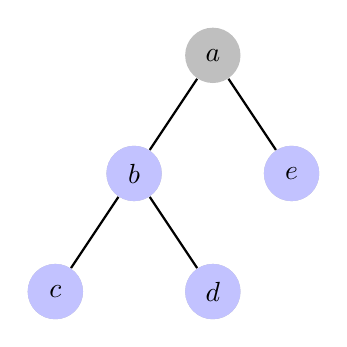
\begin{tikzpicture} [
                scale=1,
                vertex/.style={circle,fill=black!25,minimum size=20pt,inner sep=0pt},
                edge/.style = {draw,thick,-},
                selected vertex/.style = {vertex, fill=blue!24},
            ]
            \foreach \pos/\name in {
                    {(0,0)/c}, {(2,0)/d}, {(1,1.5)/b}, {(3,1.5)/e}, {(2,3)/a}}
                \node[vertex] (\name) at \pos {$\name$};
            \foreach \source/ \dest in {
                    b/c,b/d,a/b,a/e}
                \path[edge] (\source) edge (\dest);
            \foreach \vertex in {b,c,d,e}
                \path node[selected vertex] at (\vertex) {$\vertex$};
        \end{tikzpicture}
    \end{subfigure}
    \quad
    %%%%%%%%%%%%%%%%%%%%%%%%%%%%%%%%%%%%%%%%%%%%%%%%%%%%%%%%%%%%%%%%%%%%%%%%%%%%%%%%%%%%%
    \begin{subfigure}[b]{0.45\textwidth}
        \centering
        \caption{Sottografo (completo) indotto dai nodi dispari, e matching perfetto di costo minimo evidenziato}
        \label{fig:mchristmatching}
        \begin{tikzpicture} [
                scale=1,
                vertex/.style={circle,fill=black!25,minimum size=20pt,inner sep=0pt},
                edge/.style = {draw,thick,-},
                selected edge/.style = {draw,line width=5pt,-,blue!24},
            ]
            \foreach \pos/\name in {
                    {(0,0)/c}, {(2,0)/d}, {(1,1.5)/b}, {(3,1.5)/e}}
                \node[vertex] (\name) at \pos {$\name$};
            \foreach \source/ \dest in {
                    b/c,b/d,b/e,c/e,c/d,e/d}
                \path[edge] (\source) edge (\dest);
            \begin{pgfonlayer}{background}
                \foreach \source / \dest in {b/c,d/e}
                    \path[selected edge] (\source.center) -- (\dest.center);
            \end{pgfonlayer}
        \end{tikzpicture}
    \end{subfigure}
\end{figure}
    % \\[2pt]
% magic to split a figure https://tex.stackexchange.com/a/278748
\begin{figure}[htb]\ContinuedFloat
    \caption{Algoritmo di Christofides splittato in due pagine (cont.)}
    %%%%%%%%%%%%%%%%%%%%%%%%%%%%%%%%%%%%%%%%%%%%%%%%%%%%%%%%%%%%%%%%%%%%%%%%%%%%%%%%%%%%%
    \begin{subfigure}[b]{0.45\textwidth}
        \centering
        \caption{Ciclo Euleriano
            $ \langle c,b,d,e,a,b,c \rangle$
        }
        \label{fig:mchristeulertour}
        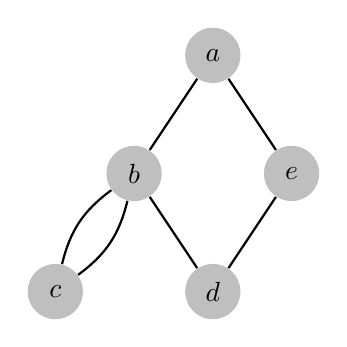
\begin{tikzpicture} [
                scale=1,
                vertex/.style={circle,fill=black!25,minimum size=20pt,inner sep=0pt},
                edge/.style = {draw,thick,-},
                bent right/.style = {bend right=20},
            ]
            \foreach \pos/\name in {
                    {(0,0)/c}, {(2,0)/d}, {(1,1.5)/b}, {(3,1.5)/e}, {(2,3)/a}}
                \node[vertex] (\name) at \pos {$\name$};
            \foreach \source/ \dest in {
                    b/d,a/b,a/e,d/e}
                \path[edge] (\source) edge (\dest);
            \foreach \source/ \dest in {
                    c/b,b/c}
                \path[edge] (\source) edge [bent right] (\dest);
        \end{tikzpicture}
    \end{subfigure}
    \quad
    %%%%%%%%%%%%%%%%%%%%%%%%%%%%%%%%%%%%%%%%%%%%%%%%%%%%%%%%%%%%%%%%%%%%%%%%%%%%%%%%%%%%%
    \begin{subfigure}[b]{0.45\textwidth}
        \centering
        \caption{Dopo lo \emph{shortcutting}:
            $ \langle c,b,d,e,a,\cancel{b},c \rangle$
        }
        \label{fig:mchristresult}
        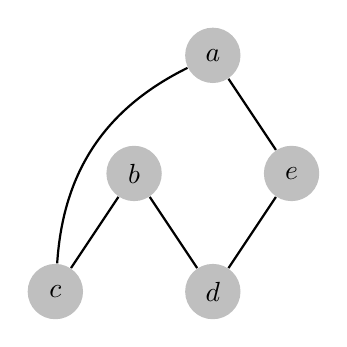
\begin{tikzpicture} [
                scale=1,
                vertex/.style={circle,fill=black!25,minimum size=20pt,inner sep=0pt},
                edge/.style = {draw,thick,-},
                bent right/.style = {bend right=30},
            ]
            \foreach \pos/\name in {
                    {(0,0)/c}, {(2,0)/d}, {(1,1.5)/b}, {(3,1.5)/e}, {(2,3)/a}}
                \node[vertex] (\name) at \pos {$\name$};
            \foreach \source/ \dest in {
                    b/d,a/e,d/e,b/c}
                \path[edge] (\source) edge (\dest);
            \foreach \source/ \dest in {
                    a/c}
                \path[edge] (\source) edge [bent right] (\dest);
        \end{tikzpicture}
    \end{subfigure}
\end{figure}

\lipsum{10}

\begin{figure}[h]
    \centering
    \caption{$3-CNF-SAT$ to $CLIQUE$}
    \label{fig:3cnfsatex}
    \begin{tikzpicture} [
            scale=1,
            vertex/.style={circle,fill=black!25,minimum size=20pt,inner sep=0pt},
            edge/.style = {draw,thin,-},
            outbound edge/.style = {draw,line width=4pt,-,blue!30},
            selected edge/.style = {draw,line width=4pt,-,red!30},
        ]
        % First we draw the vertices
        \foreach \pos/\name/\label in {
                % top left
                {(-1.5,5)/c/x_3},
                {(-2.5,3.5)/b/x_2},
                {(-3.5,2)/a/\bar{x_1}},
                % top right
                {(1.5,5)/d/x_1},
                {(2.5,3.5)/e/x_2},
                {(3.5,2)/f/\bar{x_3}},
                % bottom row
                {(2,0)/g/\bar{x_3}},
                {(0,0)/h/\bar{x_2}},
                {(-2,0)/i/x_1}}
            \node[vertex] (\name) at \pos {\name $\label$};
        % Connect vertices with edges
        \foreach \source/ \dest in {
                f/g,f/i,
                e/g,e/i,
                d/g,d/h,d/i,
                c/d,c/e,c/h,c/i,
                b/d,b/e,b/f,b/g,b/i,
                a/e,a/f,a/g,a/h}
            \path[edge] (\source) -- (\dest);
        % color some edges on background layer
        \begin{pgfonlayer}{background}
            \foreach \source / \dest in {c/d,d/i,i/c}
                \path[outbound edge] (\source.center) -- (\dest.center);
            \foreach \source / \dest in {a/e,e/g,g/a}
                \path[selected edge] (\source.center) -- (\dest.center);
        \end{pgfonlayer}
    \end{tikzpicture}
\end{figure}
